% Inspired by Bùi Vân Anh
% Begin rewrite by ledangquangdangquang on 2024-09-30
\documentclass{thesis-config}

%----- GÓI BỔ SUNG CHO BÁO CÁO -----
\usepackage{booktabs}
\usepackage{multirow}
\usepackage{pgfplots}
\pgfplotsset{compat=1.17}
\usetikzlibrary{arrows.meta, positioning, shapes.geometric, fit, backgrounds, decorations.pathreplacing}
\usepackage{xurl}      % cho phép ngắt dòng trong tên tham số dài (\nolinkurl)
\emergencystretch=2em
\usepackage{fancyvrb}  % chèn mã nguồn có chú thích tiếng Việt (listings không xử lý được UTF-8 nhiều byte)
% Ảnh "code snap" do tools/make_snaps.py sinh ra; DPI ghi trong PNG nên mọi ảnh cùng cỡ chữ
% Tiêu đề (tuỳ chọn) và ảnh nằm trong một minipage để không bị tách sang hai trang
\newcommand{\codesnap}[2][]{%
    \par\medskip\noindent\begin{minipage}{\textwidth}
        \if\relax\detokenize{#1}\relax\else\textbf{#1}\par\smallskip\fi
        \centering\includegraphics{Images/code/#2.png}
    \end{minipage}\par\medskip
}
% Ảnh chụp terminal kết quả chạy (Images/run/), tiêu đề và ảnh không bị tách trang
\newcommand{\runshot}[2][]{%
    \par\medskip\noindent\begin{minipage}{\textwidth}
        \textit{#1}\par\smallskip
        \centering\includegraphics[width=0.85\textwidth]{Images/run/#2.png}
    \end{minipage}\par\medskip
}
% Khung giữ chỗ cho ảnh chụp sẽ bổ sung sau khi chạy thí nghiệm
\newcommand{\placeholderfig}[4]{%
    \begin{figure}[H]
        \centering
        \fbox{\parbox[c][#1][c]{0.9\textwidth}{\centering\itshape\small #2}}
        \caption[#3]{\textit{\fontsize{12pt}{0}\selectfont #3}}
        \label{#4}
    \end{figure}
}

%----- PERSONAL INFORMATION -----
\title{Đánh giá chi phí mạng của Federated Learning tại biên: băng thông, độ trễ đồng bộ và điểm nghẽn tại Aggregation Node trong kiến trúc Edge--Cloud}
\author{Nhóm [số nhóm]}
\specialization{Hướng 2: Networking for AI}
\authoremail{[email nhóm]}
\universitycity{HÀ NỘI}
\university{ĐẠI HỌC BÁCH KHOA HÀ NỘI}
\school{[Tên trường/khoa]}
\department{Hệ thống và mạng máy tính (MI4060)}
\classcode{[Mã lớp]}
\advisor{Ngô Thị Hiền}
\makeatletter\newcommand{\theadvisor}{\@advisor}\makeatother
\degree{Báo cáo bài tập lớn}
\degreemonth{\the\month}
\degreeyear{\the\year}
\major{}
\members{
    & [Họ tên thành viên 1] & [MSSV] \\[1ex]
    & [Họ tên thành viên 2] & [MSSV] \\[1ex]
    & [Họ tên thành viên 3] & [MSSV] \\[1ex]
    & [Họ tên thành viên 4] & [MSSV] \\[1ex]
    & [Họ tên thành viên 5] & [MSSV] \\[1ex]
    & [Họ tên thành viên 6] & [MSSV] \\[1ex]
}

%----- MAIN DOCUMENT -----
\begin{document}
    % MỞ ĐẦU
    % Bìa ở trong file thesis-config.cls
% \maketitle % Bìa cho đồ án cá nhân
\groupTitle % Bìa cho báo cáo nhóm; danh sách thành viên khai báo bằng \members trong project_htmmt.tex

    \thispagestyle{empty}

\subsection*{\centering Lời cảm ơn}
Nhóm xin cảm ơn cô \theadvisor{} đã góp ý cho đề tài trong quá trình đăng ký và thực hiện. Các sai sót còn lại trong báo cáo thuộc trách nhiệm của nhóm.

\subsection*{\centering Tóm tắt nội dung}
Trong Federated Learning (FL), các thiết bị biên không gửi dữ liệu thô mà gửi tham số mô hình về một nút tổng hợp sau mỗi vòng huấn luyện. Khi mô hình có kích thước hàng chục MB và số nút tăng, đường lên nút tổng hợp trở thành chỗ quyết định thời gian của cả vòng. Báo cáo này xét chi phí mạng của quá trình đồng bộ đó mà không huấn luyện mô hình thật: mỗi Edge Node chỉ truyền một khối dữ liệu kích thước cố định (10 MB, tương ứng một checkpoint) lặp lại qua nhiều vòng.

Hệ thống được dựng trên Mininet gồm 2--6 Edge Node, một Edge Switch, một Edge Aggregator đặt cạnh switch và một Cloud Server nằm sau liên kết WAN có giới hạn băng thông và độ trễ. Nhóm tự định nghĩa giao thức ứng dụng FLSync chạy trên TCP, viết client/server bằng Python và bắt gói bằng tcpdump/Wireshark để phân tích bắt tay, slow start và cửa sổ trượt. Ba câu hỏi đặt ra: (1) thời gian một vòng thay đổi thế nào khi số nút tăng từ 2 lên 6; (2) nén bản cập nhật xuống 1/10 giảm thời gian truyền và RTT khi có tải bao nhiêu; (3) tổng hợp tại biên so với trên cloud chênh nhau bao nhiêu do RTT chặng WAN.

Mô hình giải tích của nhóm dự đoán thời gian truyền tăng gần tuyến tính theo số nút (khoảng 0{,}84~s cho mỗi nút với 10 MB trên link 100 Mbps), nén 1/10 giảm gần đúng 10 lần ở biên nhưng chỉ khoảng 3{,}6 lần với một nút khi đi qua WAN 44 ms vì slow start chiếm phần lớn thời gian, và khi WAN chỉ có 20 Mbps thì thời gian vòng ở Cloud gấp khoảng 4{,}6 lần ở Edge, gần như toàn bộ do băng thông. Số đo trên Mininet xác nhận link tới Aggregator bão hoà ở 91--95 Mbps và tỷ lệ Cloud/Edge khoảng 4{,}9 lần khi WAN 20 Mbps; nén chiều lên rút ngắn vòng 36--38\% ở 6 nút. Sai khác chính so với mô hình đến từ việc các pha tải xuống và upload chồng lên nhau, và từ mất gói tại hàng đợi chặng WAN.

Đề tài đăng ký Hướng 2 (Networking for AI).

\vfill
\begin{tabularx}{\textwidth}{>{\centering\arraybackslash}X>{\centering\arraybackslash}X}
    \centering
    & Đại diện nhóm thực hiện \\
    \centering
    &\fontsize{10pt}{0}\selectfont Ký và ghi rõ họ tên \\
    \centering
\end{tabularx}

\cleardoublepage

    % MỤC LỤC
\addtocontents{toc}{\protect\thispagestyle{empty}}
\tableofcontents % tạo mục lục tự dộng 
\thispagestyle{empty}
\cleardoublepage







    \pagenumbering{roman} % Đánh số trang thứ tự la mã
    \phantomsection\section*{\centering DANH MỤC KÝ HIỆU VÀ CHỮ VIẾT TẮT}
\addcontentsline{toc}{section}{\numberline {} DANH MỤC KÝ HIỆU VÀ CHỮ VIẾT TẮT}
\begin{longtable}{ @{} p{4.6cm} p{9.9cm} @{} }
ACK & Acknowledgement -- gói/cờ xác nhận \\
AQM & Active Queue Management -- quản lý hàng đợi chủ động (ví dụ CoDel) \\
BDP & Bandwidth--Delay Product -- tích băng thông và độ trễ \\
cwnd & Congestion window -- cửa sổ tắc nghẽn của TCP \\
FedAvg & Federated Averaging -- thuật toán tổng hợp trung bình có trọng số \\
FL & Federated Learning -- học liên kết \\
HTB & Hierarchical Token Bucket -- bộ định hình lưu lượng của Linux \\
IW & Initial Window -- cửa sổ khởi đầu của TCP \\
MLP & Multi-Layer Perceptron -- mạng nơ-ron truyền thẳng nhiều lớp \\
MSS & Maximum Segment Size -- kích thước đoạn TCP tối đa \\
MTU & Maximum Transmission Unit \\
NIC & Network Interface Card \\
OVS & Open vSwitch \\
RTO & Retransmission Timeout -- thời gian chờ trước khi truyền lại \\
RTT & Round-Trip Time -- thời gian khứ hồi \\
rwnd & Receive window -- cửa sổ nhận \\
SGD & Stochastic Gradient Descent -- hạ gradient ngẫu nhiên \\
TCP & Transmission Control Protocol \\
TTA & Time-to-Accuracy -- thời gian để mô hình đạt độ chính xác mục tiêu \\
WAN & Wide Area Network \\[2ex]
$S$ & Kích thước payload một bản mô hình/cập nhật (byte) \\
$N$ & Số Edge Node tham gia một vòng \\
$B$ & Băng thông link nghẽn (bit/s) \\
$\eta$ & Hiệu suất tải tin của một khung Ethernet \\
$p$ & Tỉ lệ mất gói mỗi chiều của chặng WAN \\
$K$ & Số vòng cần để đạt độ chính xác mục tiêu \\
$R$ & RTT cơ sở của đường đi (không có hàng đợi) \\
$d_{trans}, d_{prop}, d_{queue}, d_{proc}$ & Trễ truyền, trễ lan truyền, trễ hàng đợi, trễ xử lý \\
$T_{down}, T_{up}, T_{round}$ & Thời gian pha phát mô hình, pha thu cập nhật, cả vòng \\
\end{longtable}
\cleardoublepage

    % DANH MỤC HÌNH VẼ
\phantomsection
{
    \let\oldnumberline\numberline%
    \renewcommand{\numberline}{\figurename~\oldnumberline}%
    \listoffigures%
}
\addcontentsline{toc}{section}{\numberline {} DANH MỤC HÌNH VẼ}
\cleardoublepage
    % DANH MỤC BẢNG BIỂU
\phantomsection
{
    \let\oldnumberline\numberline%
    \renewcommand{\numberline}{\tablename~\oldnumberline}%
    \listoftables%
}
\addcontentsline{toc}{section}{\numberline {} DANH MỤC BẢNG BIỂU}
\cleardoublepage
    \pagenumbering{arabic}% Đánh số trang thứ tự bình thường
    % NỘI DUNG
    \chaptercustom{1}{CƠ SỞ LÝ THUYẾT}
\setcounter{section}{1}
\setcounter{equation}{0}
Chương này trình bày các kiến thức cần cho việc thiết kế thí nghiệm và giải thích kết quả: kiến trúc Edge--Cloud và điện toán biên, quy trình một vòng Federated Learning cùng lưu lượng mà nó sinh ra, mô hình phân tầng mạng và các cơ chế của TCP ảnh hưởng tới việc truyền một khối dữ liệu lớn, các chỉ số đo hiệu năng mạng, và các công cụ dùng để giả lập, lập trình và phân tích gói tin.

%=====================================================================
\subsection{Tổng quan kiến trúc Edge--Cloud và Điện toán biên}
\label{sec:1-1}

\subsubsection{Từ mô hình Cloud tập trung tới Edge Computing}
Trong mô hình điện toán đám mây tập trung, thiết bị đầu cuối gửi dữ liệu về trung tâm dữ liệu để xử lý rồi nhận lại kết quả. Mô hình này có tài nguyên tính toán lớn và dễ quản lý, nhưng mọi yêu cầu đều phải đi qua mạng diện rộng (WAN): RTT tới trung tâm dữ liệu thường lên tới hàng chục ms, băng thông đường lên của thiết bị bị giới hạn, và lưu lượng từ hàng nghìn thiết bị dồn về lõi mạng.

Edge computing (điện toán biên) đưa một phần năng lực tính toán và lưu trữ tới gần nguồn sinh dữ liệu, ví dụ một máy chủ đặt ở trạm gốc, ở phòng máy của toà nhà hay trong mạng nội bộ của nhà máy \cite{shi2016edge}. Dữ liệu được xử lý ngay tại biên, chỉ kết quả đã rút gọn mới được gửi lên cloud. Lợi ích chính là độ trễ thấp hơn, giảm lưu lượng lên lõi mạng và giữ dữ liệu nhạy cảm ở gần chủ sở hữu.

\subsubsection{Đặc thù của hệ thống Edge--Cloud}
Kiến trúc Edge--Cloud kết hợp hai tầng: các nút biên gần thiết bị và cloud ở xa. Hệ thống loại này có các đặc thù của một hệ phân tán:
\begin{itemize}
    \item \textbf{Nhiều nút, phân tán về vị trí.} Dữ liệu và tính toán nằm rải rác trên nhiều Edge Node; không nút nào có toàn bộ thông tin.
    \item \textbf{Liên kết không đồng nhất.} Trong vùng biên, các nút nối với nhau qua LAN có RTT vài ms và băng thông cao. Giữa vùng biên và cloud là chặng WAN có RTT lớn hơn một bậc và băng thông thường thấp hơn LAN.
    \item \textbf{Cần đồng bộ.} Khi các nút cùng thực hiện một nhiệm vụ chung (như huấn luyện một mô hình), chúng phải trao đổi trạng thái định kỳ; tốc độ của cả hệ thống bị giới hạn bởi nút và liên kết chậm nhất.
    \item \textbf{Điểm tập trung lưu lượng.} Nút điều phối (gateway, nút tổng hợp) nhận lưu lượng của mọi nút biên nên dễ trở thành điểm nghẽn.
\end{itemize}

Bảng~\ref{tab:edgecloud} so sánh hai vị trí đặt nút xử lý trung tâm.

\begin{table}[H]
    \centering
    \caption{So sánh đặt nút xử lý tại biên và trên cloud}
    \label{tab:edgecloud}
    \begin{tabularx}{\textwidth}{>{\raggedright\arraybackslash\hsize=0.6\hsize}X >{\raggedright\arraybackslash\hsize=1.2\hsize}X >{\raggedright\arraybackslash\hsize=1.2\hsize}X}
        \toprule
        \textbf{Tiêu chí} & \textbf{Tại biên (Edge)} & \textbf{Trên cloud} \\
        \midrule
        Vị trí & Cùng mạng cục bộ với Edge Node & Trung tâm dữ liệu, sau chặng WAN \\
        \midrule
        RTT & Vài ms & Hàng chục ms trở lên \\
        \midrule
        Băng thông & Bằng mạng LAN biên & Bị giới hạn bởi chặng WAN \\
        \midrule
        Tài nguyên tính toán & Hạn chế & Lớn, dễ mở rộng \\
        \midrule
        Phạm vi dữ liệu & Chỉ các nút trong vùng & Mọi vùng biên \\
        \bottomrule
    \end{tabularx}
\end{table}

Hai vị trí này có thể kết hợp. Kiến trúc phân cấp client--edge--cloud HierFAVG \cite{liu2020hierfavg} tổng hợp nhiều lần ở biên rồi mới gửi một bản lên cloud. Lim và cộng sự tổng kết các hướng giảm chi phí truyền thông khi đưa học máy phân tán vào mạng biên \cite{lim2020survey}. Đề tài này dựng cả hai vị trí trên cùng một topo (Mục~\ref{sec:2-3}) để so sánh trực tiếp.

%=====================================================================
\subsection{Tổng quan về Federated Learning (FL)}
\label{sec:1-2}

\subsubsection{Khái niệm và quy trình một vòng}
Federated Learning (FL) được McMahan và cộng sự đề xuất năm 2017 như một cách huấn luyện mô hình học máy trên dữ liệu phân tán mà không phải gom dữ liệu thô về một nơi \cite{mcmahan2017fedavg}. Hệ thống gồm một nút tổng hợp (aggregator, server) và nhiều máy khách (client) giữ dữ liệu riêng. Quá trình huấn luyện gồm nhiều vòng (aggregation round); mỗi vòng có bốn bước:
\begin{enumerate}
    \item Nút tổng hợp phát tham số mô hình toàn cục $w_t$ xuống $N$ máy khách (chiều xuống).
    \item Mỗi máy khách huấn luyện vài epoch trên dữ liệu cục bộ, thu được $w_{t+1}^{k}$.
    \item Máy khách gửi tham số mới, hoặc độ chênh tham số (gradient, $w_{t+1}^{k} - w_t$), về nút tổng hợp (chiều lên).
    \item Nút tổng hợp kết hợp các bản cập nhật thành mô hình toàn cục mới và bắt đầu vòng sau.
\end{enumerate}

\subsubsection{Thuật toán FedAvg}
Trong thuật toán FedAvg \cite{mcmahan2017fedavg}, máy khách $k$ có $n_k$ mẫu dữ liệu. Nút tổng hợp lấy trung bình có trọng số:
\begin{equation}
    w_{t+1} = \sum_{k=1}^{N} \frac{n_k}{n}\, w_{t+1}^{k}, \qquad n = \sum_{k=1}^{N} n_k
    \label{eq:fedavg}
\end{equation}
Phép tổng hợp chỉ là cộng có trọng số nên tốn rất ít thời gian so với việc truyền dữ liệu.

\subsubsection{Bài toán truyền tải trọng số giữa Edge Node và Aggregator}
Nếu mỗi bản mô hình có kích thước $S$ byte thì một vòng sinh ra $N \cdot S$ byte theo chiều xuống và $N \cdot S$ byte theo chiều lên, \emph{tất cả đều đi qua giao diện mạng của nút tổng hợp}. Đây là lý do nút tổng hợp là điểm nghẽn tự nhiên của hệ thống.

FL thường chạy đồng bộ: một vòng chỉ kết thúc khi bản cập nhật \emph{cuối cùng} tới nơi. Vì vậy thời gian vòng bằng thời gian của máy khách chậm nhất (straggler). Trong hệ thống FL của Google, Bonawitz và cộng sự xử lý việc này bằng cách chọn nhiều thiết bị hơn số cần cho mỗi vòng rồi bỏ qua các thiết bị báo cáo muộn \cite{bonawitz2019towards}.

Để giảm lưu lượng, có thể nén bản cập nhật: lượng tử hoá, hoặc chỉ gửi các phần tử gradient lớn nhất. Deep Gradient Compression báo cáo mức nén 270--600 lần mà không giảm độ chính xác \cite{lin2018dgc}. Đề tài chọn mức nén 1/10 như một giá trị thận trọng và chỉ quan tâm tới tác động của nó lên mạng.

%=====================================================================
\subsection{Nền tảng mạng máy tính và giao thức truyền tải TCP}
\label{sec:1-3}

\subsubsection{Mô hình phân tầng OSI và TCP/IP}
Mô hình OSI chia chức năng truyền thông thành bảy tầng; bộ giao thức TCP/IP dùng trên Internet gộp lại thành bốn tầng \cite{kurose2021computer}. Mỗi tầng chỉ dùng dịch vụ của tầng ngay dưới và thêm header của mình vào dữ liệu nhận từ tầng trên (đóng gói, encapsulation). Bảng~\ref{tab:osi} đối chiếu hai mô hình và chỉ ra giao thức tương ứng trong hệ thống của đề tài.

\begin{table}[H]
    \centering
    \caption{Đối chiếu mô hình OSI, TCP/IP và các giao thức trong đề tài}
    \label{tab:osi}
    \begin{tabularx}{\textwidth}{>{\raggedright\arraybackslash\hsize=0.8\hsize}X >{\raggedright\arraybackslash\hsize=0.7\hsize}X >{\raggedright\arraybackslash\hsize=0.6\hsize}X >{\raggedright\arraybackslash\hsize=1.9\hsize}X}
        \toprule
        \textbf{Tầng OSI} & \textbf{Tầng TCP/IP} & \textbf{Đơn vị dữ liệu} & \textbf{Trong đề tài} \\
        \midrule
        7 Ứng dụng, 6 Trình diễn, 5 Phiên & Ứng dụng & Thông điệp & Giao thức FLSync (header 20 byte, tuần tự hoá big-endian) \\
        \midrule
        4 Giao vận & Giao vận & Đoạn (segment) & TCP cổng 5000, MSS 1460 byte \\
        \midrule
        3 Mạng & Mạng (Internet) & Gói (packet) & IPv4, định tuyến qua Edge Gateway \texttt{r1}, lọc gói bằng iptables \\
        \midrule
        2 Liên kết dữ liệu, 1 Vật lý & Truy nhập mạng & Khung (frame) & Ethernet qua Open vSwitch và cặp giao diện ảo \texttt{veth} \\
        \bottomrule
    \end{tabularx}
\end{table}

Khi một thông điệp FLSync 10 MB đi xuống các tầng, TCP chia nó thành nhiều đoạn vừa với MSS, IP thêm header 20 byte và Ethernet thêm header 14 byte. Hình~\ref{fig:encap} ở Mục~\ref{sec:2-4} minh hoạ chi tiết quá trình này.

\subsubsection{Bắt tay ba bước}
TCP \cite{rfc9293} là giao thức hướng kết nối, tin cậy, truyền luồng byte có thứ tự. Kết nối được thiết lập bằng bắt tay ba bước: bên khởi tạo gửi SYN, bên nhận trả SYN-ACK, bên khởi tạo gửi ACK. Bên khởi tạo chỉ gửi được dữ liệu sau một RTT. Trong lúc bắt tay hai bên trao đổi các tuỳ chọn: MSS (mặc định 1460 byte trên Ethernet), Window Scale, SACK Permitted và Timestamps. Khi dùng Timestamps, mỗi đoạn mang thêm 12 byte tuỳ chọn nên phần tải tin thực tế còn 1448 byte. Kết nối được đóng bằng trao đổi FIN theo cả hai chiều.

\subsubsection{Cửa sổ trượt và điều khiển luồng}
Bên gửi được phép có tối đa $\min(cwnd, rwnd)$ byte đang bay (đã gửi, chưa được xác nhận). $rwnd$ do bên nhận quảng bá theo chỗ trống bộ đệm; $cwnd$ do bên gửi tự điều chỉnh theo tình trạng mạng. Thông lượng tối đa của một luồng xấp xỉ:
\begin{equation}
    \text{Thông lượng} \approx \frac{\min(cwnd, rwnd)}{RTT}
    \label{eq:tput}
\end{equation}
Để lấp đầy link, cửa sổ phải đạt ít nhất tích băng thông--độ trễ:
\begin{equation}
    BDP = B \cdot RTT
    \label{eq:bdp}
\end{equation}
Với $B = 100$ Mbps và các RTT của topo ở Mục~\ref{sec:2-3}: ở biên ($RTT = 4$~ms) $BDP = 50$~KB; qua WAN ($RTT = 44$~ms) $BDP = 550$~KB.

\subsubsection{Điều khiển tắc nghẽn và TCP Slow Start}
RFC 5681 \cite{rfc5681} quy định hai pha chính. Trong slow start, $cwnd$ bắt đầu từ cửa sổ khởi đầu IW và tăng thêm một MSS cho mỗi ACK, tức là gấp đôi sau mỗi RTT. Linux dùng $IW = 10$ MSS theo RFC 6928 \cite{rfc6928}, khoảng 14{,}5~KB. Khi gặp mất gói hoặc vượt ngưỡng $ssthresh$, TCP chuyển sang pha tránh tắc nghẽn; Linux mặc định dùng thuật toán CUBIC \cite{rfc9438} cho pha này.

Số RTT cần để $cwnd$ từ IW đạt BDP là:
\begin{equation}
    k^{*} = \left\lceil \log_2 \frac{BDP}{IW} \right\rceil
    \label{eq:kstar}
\end{equation}
Ở biên, $k^{*} = \lceil \log_2(50/14{,}5) \rceil = 2$ RTT, tức 8~ms, bỏ qua được. Qua WAN, $k^{*} = \lceil \log_2(550/14{,}5) \rceil = 6$ RTT, tức 264~ms. Với khối 10 MB truyền mất gần 1~s, 264~ms này chiếm khoảng một phần tư; với khối 1 MB, phần lớn thời gian truyền nằm trong slow start.

Ở FL, giữa hai lần gửi luôn có khoảng nghỉ huấn luyện. RFC 5681 (mục 4.1) khuyến nghị đặt lại $cwnd$ về cửa sổ khởi động lại nếu kết nối nghỉ lâu hơn một RTO; Linux bật mặc định qua tham số \nolinkurl{net.ipv4.tcp_slow_start_after_idle = 1}. Do đó \emph{dù giữ kết nối TCP lâu dài, mỗi vòng FL vẫn phải trả lại chi phí slow start}. Bản bắt gói ở Hình~\ref{fig:ws-stevens} (Mục~\ref{sec:2-7}) xác nhận điều này: đầu vòng 2, luồng lại bắt đầu từ IW = 10 gói.

\subsubsection{Chia sẻ băng thông giữa các luồng}
Khi $N$ luồng TCP có cùng RTT đi qua một link nghẽn, cơ chế điều khiển tắc nghẽn đưa mỗi luồng về xấp xỉ $B/N$. Hệ quả là các Edge Node kết thúc gần như cùng lúc, và thời gian truyền $N$ khối gần bằng thời gian truyền một khối lớn gấp $N$ lần, xấp xỉ $8NS/(\eta B)$ khi khối đủ lớn.

\subsubsection{Thông lượng TCP khi có mất gói ngẫu nhiên}
Khi đường truyền mất gói ngẫu nhiên với tỉ lệ $p$, mỗi lần mất gói TCP giảm cửa sổ tắc nghẽn, nên cửa sổ không còn lấp đầy được link. Mathis và cộng sự chỉ ra rằng thông lượng trung bình của một luồng TCP khi đó xấp xỉ \cite{mathis1997macroscopic}:
\begin{equation}
    X(p, R) \approx \frac{MSS}{R}\sqrt{\frac{3}{2p}}
    \label{eq:mathis}
\end{equation}
với $R$ là RTT. Công thức cho thấy thông lượng giảm theo $1/\sqrt{p}$ và tỉ lệ nghịch với RTT, nên mất gói gây hại nhiều hơn khi nút tổng hợp ở xa. Công thức bỏ qua timeout (RTO), vốn xuất hiện nhiều khi $p$ lớn, nên thời gian truyền thực tế thường dài hơn giá trị suy ra từ~\eqref{eq:mathis}.

%=====================================================================
\subsection{Các chỉ số đo lường hiệu năng mạng (Network Metrics)}
\label{sec:1-4}

\subsubsection{Các thành phần độ trễ của một gói}
Theo Kurose và Ross (mục 1.4) \cite{kurose2021computer}, độ trễ của một gói tại mỗi nút gồm bốn thành phần:
\begin{equation}
    d_{nodal} = d_{proc} + d_{queue} + d_{trans} + d_{prop}
    \label{eq:dnodal}
\end{equation}
trong đó:
\begin{itemize}
    \item $d_{proc}$: thời gian xử lý header, tra bảng chuyển tiếp; cỡ micro giây, bỏ qua được.
    \item $d_{queue}$: thời gian chờ trong hàng đợi đầu ra; phụ thuộc mức tải.
    \item $d_{trans} = L/R$: thời gian đẩy toàn bộ $L$ bit của gói lên đường truyền tốc độ $R$.
    \item $d_{prop} = d/s$: thời gian tín hiệu lan truyền trên quãng đường $d$ với tốc độ $s$.
\end{itemize}

Với một khối 10 MB (80 Mbit) qua link 100 Mbps, riêng $d_{trans}$ của cả khối đã là 0{,}8~s, lớn hơn rất nhiều so với $d_{prop}$ của một link WAN điển hình (vài chục ms). Vì vậy với khối lớn, băng thông là yếu tố chính; với khối nhỏ, RTT và số vòng khứ hồi mới là yếu tố chính. Câu hỏi Q1 (quét băng thông 1--100~Mbps) và Q3 (nén bản cập nhật, vị trí nút tổng hợp) khai thác đúng ranh giới này; câu hỏi Q2 xét trường hợp RTT và mất gói cùng giới hạn tốc độ của TCP.

\subsubsection{Độ trễ truyền tải các pha của vòng FL}
Ở mức ứng dụng, một vòng đồng bộ được chia thành các pha, và đề tài đo thời gian của từng pha:
\begin{itemize}
    \item $T_{down}$: thời gian phát mô hình toàn cục xuống, tính tới khi Edge Node cuối cùng nhận đủ.
    \item $T_{train}$: thời gian huấn luyện cục bộ.
    \item $T_{up}$: thời gian gửi bản cập nhật lên, tính tới khi bản cập nhật cuối cùng tới nút tổng hợp.
    \item $T_{agg}$: thời gian tổng hợp theo~\eqref{eq:fedavg}.
\end{itemize}
Nếu các pha nối tiếp nhau, thời gian một vòng là:
\begin{equation}
    T_{round} = T_{down} + T_{train} + T_{up} + T_{agg}
    \label{eq:tround}
\end{equation}
Cách lấy mốc thời gian cho từng pha trong chương trình được nêu ở Mục~\ref{sec:2-6}.

\subsubsection{Độ trễ khứ hồi (RTT)}
RTT là thời gian từ lúc gửi một gói tới lúc nhận được phản hồi cho gói đó. Khi mạng rảnh, RTT gần bằng hai lần tổng $d_{prop}$ và $d_{trans}$ của gói nhỏ trên đường đi; đây là RTT cơ sở. Khi có tải, gói phải chờ thêm trong các hàng đợi nên RTT tăng. Đề tài đo RTT bằng \texttt{ping}: lúc rảnh để kiểm tra cấu hình topo, và chạy liên tục trong lúc truyền để thấy RTT khi có tải.

\subsubsection{Thông lượng}
Thông lượng là lượng dữ liệu truyền được trong một đơn vị thời gian. Đề tài dùng thông lượng tầng ứng dụng (goodput), chỉ tính phần tải tin:
\begin{equation}
    \text{Thông lượng} = \frac{8 \cdot D}{T}
    \label{eq:goodput}
\end{equation}
với $D$ là số byte tải tin và $T$ là thời gian truyền. Do header của các tầng chiếm một phần băng thông, thông lượng ứng dụng luôn nhỏ hơn tốc độ link $B$; tỷ lệ giữa hai đại lượng là hiệu suất $\eta$ tính ở Mục~\ref{sec:2-4}. Khi $N$ luồng chia một link, ta xét cả thông lượng gộp ($8ND/T$) và phần của mỗi luồng.

\subsubsection{Nghẽn hàng đợi (Bufferbloat)}
Khi $N$ luồng cùng đi qua một link tốc độ $B$, hàng đợi tại đầu link bắt đầu đầy. Một hàng đợi chứa $Q$ gói kích thước $L$ thêm vào mỗi gói một độ trễ tối đa:
\begin{equation}
    d_{queue}^{max} = \frac{Q \cdot L}{B}
    \label{eq:dqueue}
\end{equation}
Với $Q = 200$ gói, $L = 1514$ byte và $B = 100$ Mbps, $d_{queue}^{max} \approx 24$~ms. Hiện tượng hàng đợi lớn làm RTT tăng vọt khi có tải được gọi là bufferbloat. Hàng đợi quá nhỏ thì ngược lại: gói bị bỏ thường xuyên, TCP phải truyền lại và giảm cửa sổ.

%=====================================================================
\subsection{Công cụ mô phỏng mạng và tự động hóa}
\label{sec:1-5}

\subsubsection{Mininet và Open vSwitch}
Mininet \cite{lantz2010mininet} tạo các host ảo bằng network namespace của Linux: mỗi host có bảng định tuyến, giao diện mạng và ngăn xếp TCP/IP riêng nhưng dùng chung nhân hệ điều hành. Các host được nối bằng cặp giao diện ảo \texttt{veth}. Topo có thể khai báo bằng một script Python, nên dễ tạo lại giống hệt nhau cho mỗi lần đo.

Switch trong Mininet mặc định là Open vSwitch (OVS), một switch ảo phần mềm chạy trong nhân Linux. OVS có thể hoạt động như switch OpenFlow do controller điều khiển, hoặc như một bridge L2 tự học địa chỉ MAC theo cổng vào. Đề tài dùng chế độ bridge (\texttt{OVSBridge}) vì không cần điều khiển SDN.

Lớp \texttt{TCLink} của Mininet gắn hai bộ lọc \texttt{tc} lên mỗi đầu link: HTB giới hạn tốc độ theo tham số \texttt{bw}, còn netem thêm độ trễ theo tham số \texttt{delay} và giới hạn hàng đợi theo \nolinkurl{max_queue_size}. Vì độ trễ được đặt trên \emph{mỗi đầu} của link, gói đi qua một link theo một chiều chịu đúng một lần \texttt{delay}. RTT giữa hai host bằng hai lần tổng độ trễ các link trên đường đi. Ví dụ với lệnh \texttt{sudo mn -{}-link tc,bw=10,delay=20ms}, đường h1--s1--h2 có hai link nên RTT $\approx 2 \times (20 + 20) = 80$~ms. Handigol và cộng sự đã dùng Mininet tái tạo kết quả của nhiều bài báo mạng đã công bố \cite{handigol2012reproducible}. Điều kiện là máy chạy giả lập không thiếu CPU.

\subsubsection{Lập trình Socket trong Python}
Module \texttt{socket} của Python bọc giao diện socket của hệ điều hành. Một chương trình máy chủ TCP gọi lần lượt \texttt{socket()}, \texttt{bind()}, \texttt{listen()} rồi \texttt{accept()} để nhận từng kết nối; máy khách gọi \texttt{create\_connection()} để bắt tay ba bước với máy chủ. Sau đó hai bên trao đổi dữ liệu bằng \texttt{sendall()} và \texttt{recv()}. Các điểm sau ảnh hưởng trực tiếp tới thiết kế giao thức và cách đo:
\begin{itemize}
    \item \textbf{TCP là luồng byte.} Một lần \texttt{recv()} có thể trả về một phần thông điệp hoặc phần cuối thông điệp này cùng phần đầu thông điệp sau. Ứng dụng phải tự đóng khung (framing), thường bằng một header có trường độ dài.
    \item \textbf{Tuần tự hoá header.} Module \texttt{struct} chuyển các trường số nguyên thành chuỗi byte theo định dạng cố định, ví dụ thứ tự byte mạng (big-endian) với ký hiệu \texttt{!}.
    \item \textbf{\texttt{sendall()} trả về sớm.} Hàm trả quyền khi dữ liệu đã vào bộ đệm gửi của hệ điều hành, chưa chắc đã tới đích. Muốn biết bên kia đã nhận đủ, cần một xác nhận ở tầng ứng dụng.
    \item \textbf{Thuật toán Nagle.} TCP mặc định gom các đoạn nhỏ để gửi cùng lúc. Tuỳ chọn \texttt{TCP\_NODELAY} tắt cơ chế này để thông điệp ngắn đi ngay.
    \item \textbf{Đa luồng.} Máy chủ phục vụ $N$ kết nối song song bằng module \texttt{threading}, mỗi kết nối một luồng, để các luồng TCP cùng cạnh tranh trên link như trong thực tế.
\end{itemize}

\subsubsection{Công cụ bắt và phân tích gói tin: tcpdump và Wireshark}
\texttt{tcpdump} ghi gói trên một giao diện ra file \texttt{.pcap}, có thể lọc theo giao thức, cổng và chỉ lấy một số byte đầu mỗi gói (tham số \texttt{-s}) để file nhỏ. Wireshark đọc file đó, giải mã từng tầng và cung cấp:
\begin{itemize}
    \item bộ lọc hiển thị, ví dụ \texttt{tcp.port == 5000} để chỉ xem lưu lượng FLSync, hoặc \nolinkurl{tcp.analysis.retransmission} để lọc gói truyền lại;
    \item \emph{Statistics $\rightarrow$ TCP Stream Graphs $\rightarrow$ Stevens/tcptrace}: số thứ tự theo thời gian, nhìn thấy rõ từng đợt slow start;
    \item \emph{Statistics $\rightarrow$ I/O Graphs}: thông lượng theo thời gian của từng luồng;
    \item \emph{Statistics $\rightarrow$ Conversations}: tổng byte và thời gian của mỗi kết nối.
\end{itemize}
\texttt{tshark} là bản dòng lệnh của Wireshark, dùng để trích số liệu từ file pcap bằng script (ví dụ \texttt{tshark -z io,stat,1}). Trước khi bắt gói cần tắt các cơ chế offload (TSO, GSO, GRO) trên giao diện; nếu không, tcpdump sẽ thấy các ``gói'' 64~KB do nhân ghép lại thay vì từng đoạn cỡ MSS.

%=====================================================================
\subsection{Kết luận chương}
Một vòng FL đồng bộ dồn $2NS$ byte qua giao diện của nút tổng hợp. Với khối lớn, thời gian vòng chủ yếu do $d_{trans}$ trên link nghẽn và tăng tuyến tính theo $N$. Với khối nhỏ hoặc RTT lớn, slow start (lặp lại mỗi vòng do khoảng nghỉ huấn luyện) chiếm từ một phần tư tới phần lớn thời gian truyền. Khi nhiều luồng cùng đi qua một link, hàng đợi đầy làm RTT tăng (bufferbloat). Mininet, socket Python và tcpdump/Wireshark là các công cụ để dựng, chạy và quan sát các hiện tượng này; Chương~2 dùng chúng để thiết kế và thực hiện thí nghiệm.

\cleardoublepage

    \chaptercustom{2}{CƠ SỞ LÝ THUYẾT}
\setcounter{section}{2}
\setcounter{equation}{0}
Chương này tóm tắt các kiến thức cần cho việc thiết kế thí nghiệm và giải thích kết quả: quy trình một vòng Federated Learning và lưu lượng mà nó sinh ra, kiến trúc Edge--Cloud, bốn thành phần độ trễ của một gói tin, các cơ chế của TCP ảnh hưởng tới việc truyền một khối dữ liệu lớn, và cách Mininet giả lập băng thông, độ trễ.

\subsection{Federated Learning và lưu lượng đồng bộ}
Trong thuật toán FedAvg \cite{mcmahan2017fedavg}, ở vòng $t$ máy chủ gửi tham số toàn cục $w_t$ cho $N$ máy khách. Máy khách $k$ có $n_k$ mẫu dữ liệu, huấn luyện cục bộ vài epoch để được $w_{t+1}^{k}$ rồi gửi lại. Máy chủ tổng hợp:
\begin{equation}
    w_{t+1} = \sum_{k=1}^{N} \frac{n_k}{n}\, w_{t+1}^{k}, \qquad n = \sum_{k=1}^{N} n_k
    \label{eq:fedavg}
\end{equation}

Phép tổng hợp chỉ là cộng có trọng số nên tốn rất ít thời gian so với việc truyền dữ liệu. Nếu mỗi bản mô hình có kích thước $S$ byte thì một vòng sinh ra $N \cdot S$ byte theo chiều xuống và $N \cdot S$ byte theo chiều lên, \emph{tất cả đều đi qua giao diện mạng của nút tổng hợp}. Đây là lý do nút tổng hợp là điểm nghẽn tự nhiên của hệ thống.

Một vòng chỉ kết thúc khi bản cập nhật \emph{cuối cùng} tới nơi (đồng bộ). Vì vậy thời gian vòng bằng thời gian của máy khách chậm nhất. Trong hệ thống FL của Google, Bonawitz và cộng sự xử lý việc này bằng cách chọn nhiều thiết bị hơn số cần cho mỗi vòng rồi bỏ qua các thiết bị báo cáo muộn \cite{bonawitz2019towards}.

Để giảm lưu lượng, có thể nén bản cập nhật: lượng tử hoá, chỉ gửi các phần tử gradient lớn nhất. Deep Gradient Compression báo cáo mức nén 270--600 lần mà không giảm độ chính xác \cite{lin2018dgc}. Đề tài này chọn mức nén 1/10 như một giá trị thận trọng, chỉ quan tâm tới tác động của nó lên mạng.

\subsection{Kiến trúc Edge--Cloud}
Edge computing đưa năng lực tính toán tới gần nguồn dữ liệu để giảm độ trễ và lưu lượng lên lõi mạng \cite{shi2016edge}. Với FL, nút tổng hợp có thể đặt tại biên, tức một máy chủ cùng mạng cục bộ với các Edge Node (RTT vài ms, băng thông bằng mạng LAN). Nó cũng có thể đặt trên cloud, ở trung tâm dữ liệu; khi đó mọi bản cập nhật phải đi qua liên kết WAN có RTT hàng chục ms và băng thông thường thấp hơn LAN.
Kiến trúc phân cấp HierFAVG \cite{liu2020hierfavg} kết hợp cả hai: tổng hợp nhiều lần ở biên rồi mới gửi một bản lên cloud. Lim và cộng sự tổng kết các hướng giảm chi phí truyền thông của FL trong mạng biên \cite{lim2020survey}.

\subsection{Các thành phần độ trễ}
Theo Kurose và Ross (mục 1.4) \cite{kurose2021computer}, độ trễ của một gói tại mỗi nút gồm bốn thành phần:
\begin{equation}
    d_{nodal} = d_{proc} + d_{queue} + d_{trans} + d_{prop}
    \label{eq:dnodal}
\end{equation}
trong đó:
\begin{itemize}
    \item $d_{proc}$: thời gian xử lý header, tra bảng chuyển tiếp; cỡ micro giây, bỏ qua được.
    \item $d_{queue}$: thời gian chờ trong hàng đợi đầu ra; phụ thuộc mức tải.
    \item $d_{trans} = L/R$: thời gian đẩy toàn bộ $L$ bit của gói lên đường truyền tốc độ $R$.
    \item $d_{prop} = d/s$: thời gian tín hiệu lan truyền trên quãng đường $d$ với tốc độ $s$.
\end{itemize}

Với một khối 10 MB (80 Mbit) qua link 100 Mbps, riêng $d_{trans}$ của cả khối đã là 0{,}8~s, lớn hơn rất nhiều so với $d_{prop}$ của một link WAN điển hình (vài chục ms). Vì vậy với khối lớn, băng thông là yếu tố chính; với khối nhỏ, RTT và số vòng khứ hồi mới là yếu tố chính. Câu hỏi Q2 và Q3 khai thác đúng ranh giới này.

Khi $N$ luồng cùng đi qua một link tốc độ $B$, hàng đợi tại đầu link bắt đầu đầy. Một hàng đợi chứa $Q$ gói kích thước $L$ thêm vào mỗi gói một độ trễ tối đa:
\begin{equation}
    d_{queue}^{max} = \frac{Q \cdot L}{B}
    \label{eq:dqueue}
\end{equation}
Với $Q = 200$ gói, $L = 1514$ byte và $B = 100$ Mbps, $d_{queue}^{max} \approx 24$~ms. Hiện tượng hàng đợi lớn làm RTT tăng vọt khi có tải được gọi là bufferbloat.

\subsection{Giao thức TCP}
FLSync chạy trên TCP, nên thời gian truyền một khối 10 MB phụ thuộc vào bốn cơ chế của TCP trình bày dưới đây.

\subsubsection{Thiết lập kết nối}
TCP \cite{rfc9293} thiết lập kết nối bằng bắt tay ba bước SYN, SYN-ACK, ACK. Bên khởi tạo chỉ gửi được dữ liệu sau một RTT. Trong lúc bắt tay hai bên trao đổi các tuỳ chọn: MSS (mặc định 1460 byte trên Ethernet), Window Scale, SACK Permitted và Timestamps. Khi dùng Timestamps, mỗi đoạn mang thêm 12 byte tuỳ chọn nên phần tải tin thực tế còn 1448 byte.

\subsubsection{Cửa sổ trượt và điều khiển luồng}
Bên gửi được phép có tối đa $\min(cwnd, rwnd)$ byte đang bay (đã gửi, chưa được xác nhận). $rwnd$ do bên nhận quảng bá theo chỗ trống bộ đệm; $cwnd$ do bên gửi tự điều chỉnh theo tình trạng mạng. Thông lượng tối đa của một luồng xấp xỉ:
\begin{equation}
    \text{Thông lượng} \approx \frac{\min(cwnd, rwnd)}{RTT}
    \label{eq:tput}
\end{equation}
Để lấp đầy link, cửa sổ phải đạt ít nhất tích băng thông--độ trễ:
\begin{equation}
    BDP = B \cdot RTT
    \label{eq:bdp}
\end{equation}
Với $B = 100$ Mbps: ở biên ($RTT = 4$~ms) $BDP = 50$~KB; qua WAN ($RTT = 44$~ms) $BDP = 550$~KB.

\subsubsection{Điều khiển tắc nghẽn và slow start}
RFC 5681 \cite{rfc5681} quy định hai pha chính. Trong slow start, $cwnd$ bắt đầu từ cửa sổ khởi đầu IW và tăng thêm một MSS cho mỗi ACK, tức là gấp đôi sau mỗi RTT. Linux dùng $IW = 10$ MSS theo RFC 6928 \cite{rfc6928}, khoảng 14{,}5~KB. Khi gặp mất gói hoặc vượt ngưỡng $ssthresh$, TCP chuyển sang pha tránh tắc nghẽn; Linux mặc định dùng thuật toán CUBIC \cite{rfc9438} cho pha này.

Số RTT cần để $cwnd$ từ IW đạt BDP là:
\begin{equation}
    k^{*} = \left\lceil \log_2 \frac{BDP}{IW} \right\rceil
    \label{eq:kstar}
\end{equation}
Ở biên, $k^{*} = \lceil \log_2(50/14{,}5) \rceil = 2$ RTT, tức 8~ms, bỏ qua được. Qua WAN, $k^{*} = \lceil \log_2(550/14{,}5) \rceil = 6$ RTT, tức 264~ms. Với khối 10 MB truyền mất gần 1~s, 264~ms này chiếm khoảng một phần tư; với khối 1 MB, phần lớn thời gian truyền nằm trong slow start.

Ở FL, giữa hai lần gửi luôn có khoảng nghỉ huấn luyện. RFC 5681 (mục 4.1) khuyến nghị đặt lại $cwnd$ về cửa sổ khởi động lại nếu kết nối nghỉ lâu hơn một RTO; Linux bật mặc định qua tham số \nolinkurl{net.ipv4.tcp_slow_start_after_idle = 1}. Do đó \emph{dù giữ kết nối TCP lâu dài, mỗi vòng FL vẫn phải trả lại chi phí slow start}. Bản bắt gói ở Hình~\ref{fig:ws-stevens} xác nhận điều này: đầu vòng 2, luồng lại bắt đầu từ IW = 10 gói.

\subsubsection{Chia sẻ băng thông giữa các luồng}
Khi $N$ luồng TCP có cùng RTT đi qua một link nghẽn, cơ chế điều khiển tắc nghẽn đưa mỗi luồng về xấp xỉ $B/N$. Hệ quả là các Edge Node kết thúc gần như cùng lúc, và thời gian truyền $N$ khối gần bằng thời gian truyền một khối lớn gấp $N$ lần.

\subsection{Giả lập mạng bằng Mininet}
Mininet \cite{lantz2010mininet} tạo các host ảo bằng network namespace của Linux, nối chúng bằng cặp giao diện \texttt{veth} và switch Open vSwitch. Lớp \texttt{TCLink} gắn hai bộ lọc \texttt{tc} lên mỗi đầu link: HTB giới hạn tốc độ theo tham số \texttt{bw}, còn netem thêm độ trễ theo tham số \texttt{delay} và giới hạn hàng đợi theo \nolinkurl{max_queue_size}.
Vì độ trễ được đặt trên \emph{mỗi đầu} của link, gói đi qua một link theo một chiều chịu đúng một lần \texttt{delay}. RTT giữa hai host bằng hai lần tổng độ trễ các link trên đường đi. Ví dụ với lệnh \texttt{sudo mn -{}-link tc,bw=10,delay=20ms}, đường h1--s1--h2 có hai link nên RTT $\approx 2 \times (20 + 20) = 80$~ms. Bản gợi ý đề tài ban đầu của nhóm ghi khoảng 40~ms cho lệnh này; con số 40~ms là của ví dụ \texttt{delay=10ms} trong tài liệu hướng dẫn Mininet. Handigol và cộng sự đã dùng Mininet tái tạo kết quả của nhiều bài báo mạng đã công bố, với điều kiện máy chạy giả lập không thiếu CPU \cite{handigol2012reproducible}.

\subsection{Công cụ bắt và phân tích gói}
\texttt{tcpdump} ghi gói trên một giao diện ra file \texttt{.pcap}; Wireshark đọc file đó và cung cấp:
\begin{itemize}
    \item bộ lọc hiển thị (ví dụ \texttt{tcp.port == 5000});
    \item \emph{Statistics $\rightarrow$ TCP Stream Graphs $\rightarrow$ Stevens/tcptrace}: số thứ tự theo thời gian, nhìn thấy rõ từng đợt slow start;
    \item \emph{Statistics $\rightarrow$ I/O Graphs}: thông lượng theo thời gian của từng luồng;
    \item \emph{Statistics $\rightarrow$ Conversations}: tổng byte và thời gian của mỗi kết nối.
\end{itemize}

\subsection{Kết luận chương}
Một vòng FL đồng bộ dồn $2NS$ byte qua giao diện của nút tổng hợp. Với khối lớn, thời gian vòng chủ yếu do $d_{trans}$ trên link nghẽn và tăng tuyến tính theo $N$. Với khối nhỏ hoặc RTT lớn, slow start (lặp lại mỗi vòng do khoảng nghỉ huấn luyện) chiếm từ một phần tư tới phần lớn thời gian truyền. Chương tiếp theo thiết kế topo và giao thức để đo các hiệu ứng này.

\cleardoublepage

    \chaptercustom{3}{THIẾT KẾ HỆ THỐNG VÀ PHÂN TÍCH GIAO THỨC}
\setcounter{section}{3}
\setcounter{equation}{0}
Chương này mô tả topo mạng dựng trên Mininet, giao thức ứng dụng FLSync do nhóm định nghĩa, trình tự thông điệp trong một vòng đồng bộ, và đường đi của dữ liệu qua bốn tầng application, transport, network, link. Cuối chương là kế hoạch bắt gói để lấy bằng chứng thực tế cho các phân tích.

\subsection{Topo mạng}
Hình~\ref{fig:topo} là topo dùng cho mọi kịch bản. Sáu Edge Node \texttt{h1}--\texttt{h6} nối vào Edge Switch \texttt{s1} trong mạng biên 10.0.1.0/24. Edge Aggregator \texttt{agg} nằm cùng mạng này. Để ra khỏi vùng biên, gói phải đi qua Edge Gateway \texttt{r1}: một host Linux bật chuyển tiếp IP, vừa là router giữa hai mạng, vừa là firewall (iptables). Phía bên kia liên kết WAN là mạng cloud 10.0.2.0/24 gồm switch \texttt{s2} và Cloud Server \texttt{cloud}. Số Edge Node tham gia một lần đo ($N$ = 2..6) được chọn bằng tham số dòng lệnh; các host không tham gia vẫn có mặt nhưng không phát lưu lượng.

\begin{figure}[H]
    \centering
    \begin{tikzpicture}[
        host/.style={draw, rounded corners, minimum width=1.1cm, minimum height=0.7cm, font=\small, fill=blue!8},
        sw/.style={draw, minimum width=1.1cm, minimum height=0.8cm, font=\small, fill=gray!15},
        rt/.style={draw, circle, minimum size=1.1cm, font=\small, fill=red!12},
        srv/.style={draw, rounded corners, minimum width=1.9cm, minimum height=0.9cm, font=\small, fill=orange!15, align=center},
    ]
        \foreach \i in {1,...,6} {
            \node[host] (h\i) at (0, {3.25 - (\i-1)*1.3}) {h\i};
        }
        \node[sw] (s1) at (3.2, 0) {s1};
        \foreach \i in {1,...,6} {
            \draw (h\i.east) -- (s1.west);
        }
        \node[font=\scriptsize, align=center] at (1.5, -4.2) {100 Mbps, 1 ms\\(mỗi link truy nhập)\\10.0.1.1--10.0.1.6};
        \node[srv] (agg) at (6.4, 2.4) {Edge Aggregator\\\texttt{agg} 10.0.1.100};
        \node[rt] (r1) at (6.0, -1.6) {r1};
        \node[font=\scriptsize, align=center, below=1pt of r1] {Edge Gateway\\router + firewall\\.1.254 \;|\; .2.254};
        \node[sw] (s2) at (9.9, -1.6) {s2};
        \node[srv] (cloud) at (12.8, -1.6) {Cloud Server\\\texttt{cloud} 10.0.2.200};
        \draw[very thick] (s1) -- node[font=\scriptsize, sloped, above, pos=0.45] {100 Mbps, 1 ms} (agg);
        \draw (s1) -- node[font=\scriptsize, sloped, below, pos=0.5] {100 Mbps} (r1);
        \draw[very thick, dashed] (r1) -- node[font=\scriptsize, above] {WAN, 20 ms} node[font=\scriptsize, below] {100/20 Mbps} (s2);
        \draw (s2) -- node[font=\scriptsize, above] {1 ms} (cloud);
        \begin{scope}[on background layer]
            \node[draw, dotted, rounded corners, fit=(h1)(h6)(s1)(agg), inner sep=8pt, label={[font=\small]above:Mạng biên 10.0.1.0/24}] {};
            \node[draw, dotted, rounded corners, fit=(s2)(cloud), inner sep=6pt, label={[font=\small]above:Mạng cloud 10.0.2.0/24}] {};
        \end{scope}
    \end{tikzpicture}
    \caption{Topo Edge--Cloud dùng trong thí nghiệm}
    \label{fig:topo}
\end{figure}

Vị trí và vai trò của từng thiết bị được tóm tắt trong Bảng~\ref{tab:devices}.

\begin{table}[H]
    \centering
    \caption{Thiết bị trong topo}
    \label{tab:devices}
    \begin{tabularx}{\textwidth}{l l >{\raggedright\arraybackslash}p{2.4cm} >{\raggedright\arraybackslash}X}
        \toprule
        \textbf{Thiết bị} & \textbf{Tên} & \textbf{Địa chỉ IP} & \textbf{Chức năng} \\
        \midrule
        Edge Node & \texttt{h1}--\texttt{h6} & 10.0.1.1--10.0.1.6 & Client FLSync, gửi bản cập nhật \\
        Edge Switch & \texttt{s1} & -- & Open vSwitch, chuyển mạch L2 trong mạng biên \\
        Edge Aggregator & \texttt{agg} & 10.0.1.100 & Server FLSync khi tổng hợp tại biên \\
        Router / Gateway & \texttt{r1} & 10.0.1.254, 10.0.2.254 & Định tuyến giữa mạng biên và mạng cloud; cổng mặc định của các host \\
        Firewall & \texttt{r1} (iptables) & -- & Chặn mặc định; chỉ cho TCP/5000 từ 10.0.1.0/24 tới \texttt{cloud}, ICMP echo, và gói thuộc kết nối đã mở \\
        Cloud switch & \texttt{s2} & -- & Chuyển mạch L2 trong mạng cloud \\
        Cloud Server & \texttt{cloud} & 10.0.2.200 & Server FLSync khi tổng hợp trên cloud \\
        \bottomrule
    \end{tabularx}
\end{table}

Các tham số đường truyền nằm trong Bảng~\ref{tab:params}. Băng thông WAN được đặt bằng băng thông nhánh biên (100 Mbps) trong kịch bản so sánh chính, để chênh lệch giữa Edge và Cloud chỉ còn do RTT. Kịch bản phụ hạ WAN xuống 20 Mbps cho gần với thực tế hơn.

\begin{table}[H]
    \centering
    \caption{Tham số topo và tải}
    \label{tab:params}
    \begin{tabularx}{\textwidth}{l >{\raggedright\arraybackslash}X}
        \toprule
        \textbf{Tham số} & \textbf{Giá trị} \\
        \midrule
        Link truy nhập h$_i$--s1 & 100 Mbps, 1 ms, hàng đợi 200 gói \\
        Link s1--agg (nhánh biên) & 100 Mbps, 1 ms \\
        Link s1--r1 & 100 Mbps, không thêm độ trễ \\
        Link r1--s2 (WAN) & 100 Mbps hoặc 20 Mbps, 20 ms \\
        Link s2--cloud & 100 Mbps, 1 ms \\
        RTT cơ sở tới \texttt{agg} & $2 \times (1+1) = 4$ ms \\
        RTT cơ sở tới \texttt{cloud} & $2 \times (1+0+20+1) = 44$ ms \\
        Kích thước mô hình $S$ & 10 MB ($10^7$ byte) \\
        Kích thước bản cập nhật nén & 1 MB ($10^6$ byte) \\
        Số Edge Node $N$ & 2, 3, 4, 5, 6 \\
        Thời gian huấn luyện mô phỏng & 1 s (\texttt{sleep}) \\
        Số vòng mỗi lần đo & 10 (bỏ vòng 1 khi tính trung bình) \\
        Switch & Open vSwitch ở chế độ bridge L2 (\texttt{OVSBridge}) \\
        TCP & Linux mặc định: CUBIC, IW = 10, \nolinkurl{tcp_slow_start_after_idle = 1} \\
        \bottomrule
    \end{tabularx}
\end{table}

Trước khi đo, cần kiểm tra môi trường: \texttt{h1 ping -c 10 agg} phải cho RTT khoảng 4~ms, \texttt{h1 ping -c 10 cloud} khoảng 44~ms, và \texttt{iperf} giữa \texttt{h1} và \texttt{agg} phải đạt gần 95 Mbps. Nếu iperf thấp hơn nhiều, máy ảo thiếu CPU và kết quả đo sẽ không tin cậy được.

\subsubsection{Dựng lại topo trên Cisco Packet Tracer}
Để kiểm tra phần định tuyến và firewall trên thiết bị Cisco, nhóm dựng lại cùng topo trên Cisco Packet Tracer 9.0.1 (Hình~\ref{fig:pt-topo}), giữ nguyên tên thiết bị và kế hoạch địa chỉ IP. Edge Node là PC-PT, \texttt{agg} và \texttt{cloud} là Server-PT, \texttt{s1} và \texttt{s2} là switch 2960-24TT, \texttt{r1} là router 2911 với G0/0 nối mạng biên và G0/1 nối mạng cloud. Các link đều là FastEthernet 100 Mbps, cùng băng thông với nhánh biên trên Mininet.

Packet Tracer không giả lập được độ trễ 20~ms và giới hạn 20 Mbps của chặng WAN (vốn do \texttt{tc netem} và HTB đặt trên Mininet), cũng không chạy được mã Python của FLSync. Vì vậy topo Packet Tracer chỉ dùng để kiểm tra logic mạng; mọi số đo thời gian trong báo cáo vẫn lấy từ Mininet.

\begin{figure}[H]
    \centering
    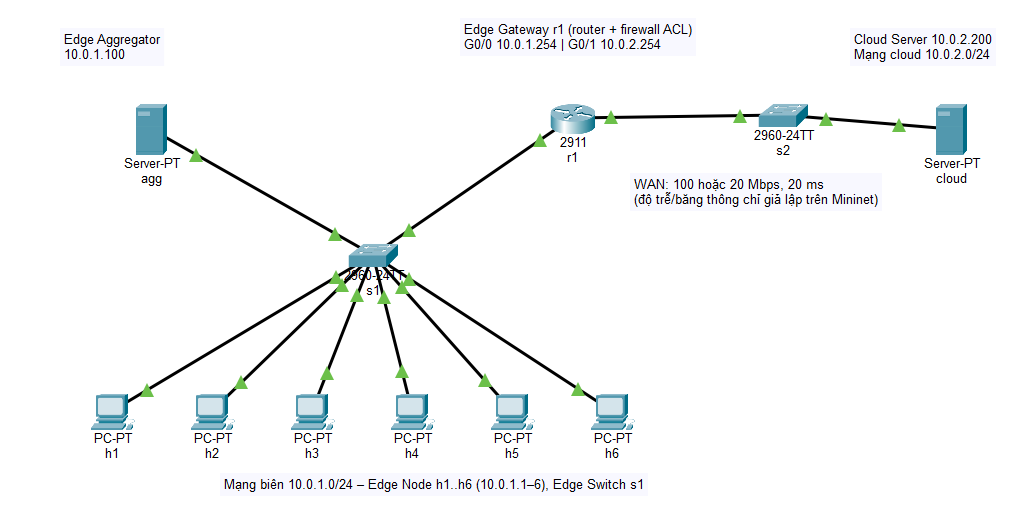
\includegraphics[width=\textwidth]{Images/pt/pt_topo.png}
    \caption{Topo Edge--Cloud dựng lại trên Cisco Packet Tracer 9.0.1}
    \label{fig:pt-topo}
\end{figure}

Firewall iptables của \texttt{r1} trên Mininet được thay bằng hai danh sách truy cập mở rộng (extended ACL) áp chiều vào trên hai cổng của router 2911:
\begin{itemize}
    \item \texttt{EDGE\_IN} trên G0/0: cho phép TCP từ 10.0.1.0/24 tới 10.0.2.200 cổng 5000 và ICMP echo, echo-reply; chặn mọi gói còn lại.
    \item \texttt{CLOUD\_IN} trên G0/1: cho phép gói TCP từ cổng 5000 của \texttt{cloud} về mạng biên khi có cờ ACK hoặc RST (từ khoá \texttt{established}, tương ứng luật \texttt{ESTABLISHED} của iptables), cùng ICMP echo, echo-reply; chặn mọi gói còn lại.
\end{itemize}
Khác với conntrack của iptables, \texttt{established} chỉ xét cờ TCP chứ không theo dõi trạng thái kết nối, nên đây là bản tương đương gần đúng.

Kết quả kiểm tra (Hình~\ref{fig:pt-test} và Hình~\ref{fig:pt-acl}):
\begin{itemize}
    \item \texttt{h1} ping \texttt{agg} (cùng mạng) nhận đủ 4/4 gói trả lời. \texttt{h1} ping \texttt{cloud} lần đầu mất 3/4 gói do ARP và cổng switch đang khởi động, các lần sau nhận đủ 4/4 với TTL = 127, tức gói đã đi qua một router.
    \item \texttt{h1} mở \texttt{http://10.0.2.200} (TCP cổng 80) thì trình duyệt báo \emph{Request Timeout}, trong khi \texttt{h2} mở được trang web của \texttt{agg} ở cùng mạng. Cổng 80 bị chặn đúng như firewall chỉ mở cổng 5000.
    \item \texttt{show access-lists} trên \texttt{r1} cho thấy luật \texttt{deny ip any any} của \texttt{EDGE\_IN} khớp 12 gói (các gói SYN HTTP bị chặn và gửi lại), luật cho ICMP echo khớp 10 gói, và luật cho echo-reply của \texttt{CLOUD\_IN} khớp 9 gói.
\end{itemize}

\begin{figure}[H]
    \centering
    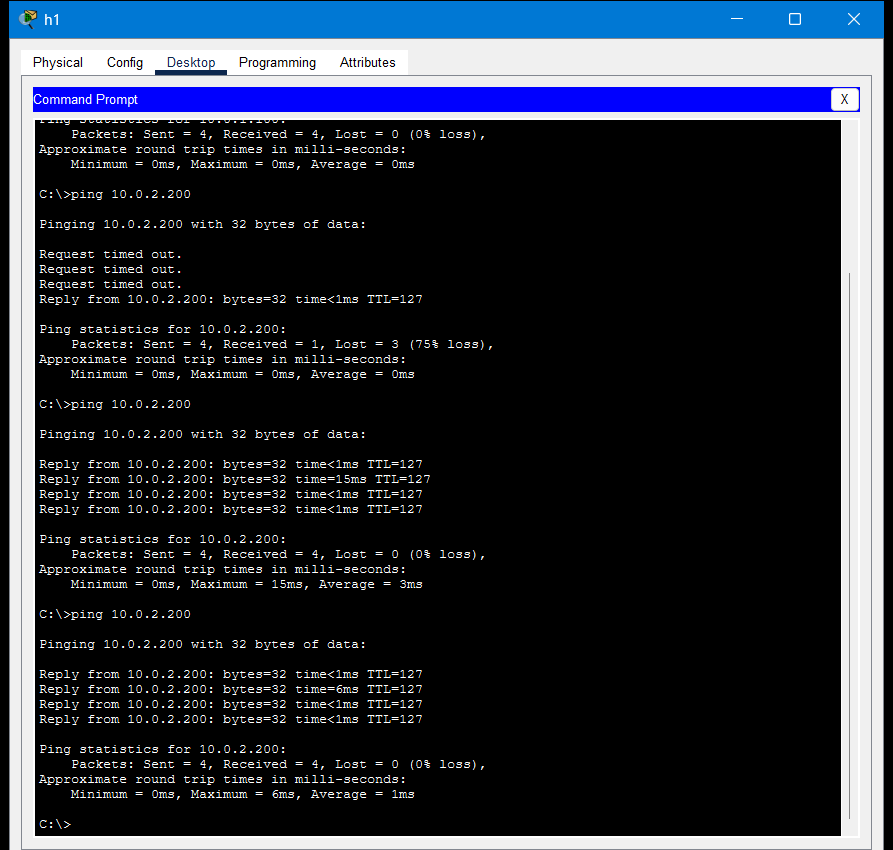
\includegraphics[width=0.62\textwidth]{Images/pt/pt_ping.png}\\[4pt]
    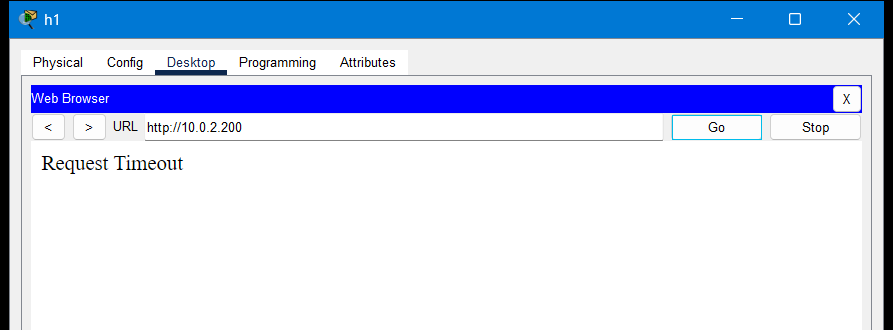
\includegraphics[width=0.62\textwidth]{Images/pt/pt_http.png}
    \caption{Packet Tracer: h1 ping Cloud Server (trên) và truy cập HTTP cổng 80 bị firewall chặn (dưới)}
    \label{fig:pt-test}
\end{figure}

\begin{figure}[H]
    \centering
    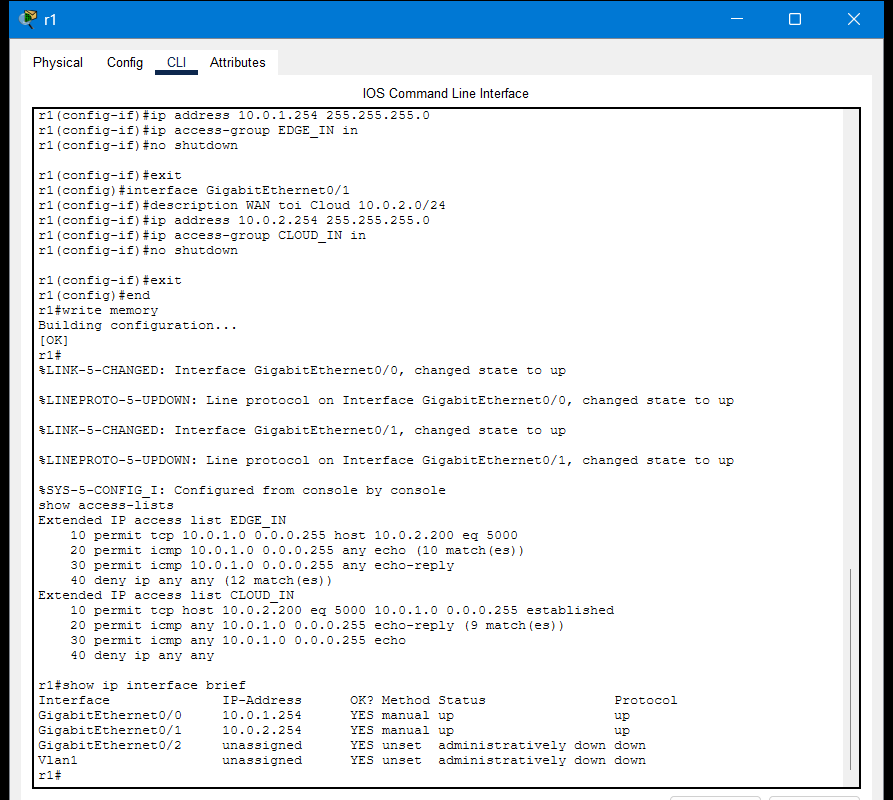
\includegraphics[width=0.75\textwidth]{Images/pt/pt_acl.png}
    \caption{Cấu hình và bộ đếm của ACL trên router r1 trong Packet Tracer}
    \label{fig:pt-acl}
\end{figure}

\subsection{Giao thức ứng dụng FLSync}
FLSync là giao thức tầng ứng dụng do nhóm viết, khoảng 50 dòng Python (\texttt{code/flproto.py}).

\subsubsection{Lý do tự định nghĩa giao thức}
gRPC hay MQTT đều chạy trên TCP và thêm các lớp đóng khung, nén header, quản lý luồng (HTTP/2) hoặc broker trung gian (MQTT). Những lớp này làm khó việc tách riêng hành vi của TCP trên bản bắt gói. Nhóm chọn một giao thức tối giản trên socket TCP để mỗi byte trên đường truyền đều giải thích được.

\subsubsection{Định dạng thông điệp}
Mỗi thông điệp gồm header cố định 20 byte (Bảng~\ref{tab:hdr}) và theo sau là phần payload có độ dài khai báo trong trường \texttt{length}. Payload là các byte 0, vì nội dung không ảnh hưởng tới mạng. Vì TCP là luồng byte không có ranh giới thông điệp, bên nhận đọc đúng 20 byte header trước, sau đó đọc đúng \texttt{length} byte.

\begin{table}[H]
    \centering
    \caption{Header của thông điệp FLSync (big-endian)}
    \label{tab:hdr}
    \begin{tabular}{l c l}
        \toprule
        \textbf{Trường} & \textbf{Byte} & \textbf{Ý nghĩa} \\
        \midrule
        \texttt{magic} & 4 & Chuỗi \texttt{FLSY}, nhận diện giao thức khi xem trên Wireshark \\
        \texttt{version} & 1 & Phiên bản, hiện là 1 \\
        \texttt{type} & 1 & 1 HELLO, 2 GLOBAL, 3 UPDATE, 4 ACK, 5 BYE \\
        \texttt{round} & 4 & Số thứ tự vòng \\
        \texttt{node} & 2 & Định danh Edge Node, 0 là server \\
        \texttt{length} & 8 & Độ dài payload (byte) \\
        \bottomrule
    \end{tabular}
\end{table}

\subsubsection{Trình tự một vòng đồng bộ}
Mỗi Edge Node mở một kết nối TCP duy nhất tới nút tổng hợp và giữ nó qua mọi vòng. Trình tự thông điệp được vẽ trên Hình~\ref{fig:seq}:
\begin{enumerate}
    \item Khởi động: client kết nối, gửi \texttt{HELLO}. Server chờ đủ $N$ client.
    \item Server gửi \texttt{GLOBAL} ($S$ byte) song song cho cả $N$ client, mỗi client một luồng.
    \item Client nhận đủ $S$ byte thì trả về \texttt{ACK} rỗng. Server dùng mốc này để đo $T_{down}$, vì hàm \texttt{sendall()} trả về ngay khi dữ liệu vào bộ đệm gửi của hệ điều hành, trước khi dữ liệu thực sự tới nơi.
    \item Client ngủ 1~s (mô phỏng huấn luyện), rồi gửi \texttt{UPDATE} ($S$ hoặc $S/10$ byte).
    \item Server nhận đủ $N$ bản \texttt{UPDATE}, tổng hợp, gửi \texttt{ACK} kết thúc vòng. $T_{round}$ tính từ lúc bắt đầu gửi \texttt{GLOBAL} tới lúc này.
    \item Sau vòng cuối, server gửi \texttt{BYE} và đóng kết nối (FIN).
\end{enumerate}

\begin{figure}[H]
    \centering
    \begin{tikzpicture}[
        msg/.style={-{Stealth[length=2.5mm]}, thick},
        note/.style={font=\scriptsize, fill=white, inner sep=1pt}
    ]
        \node[font=\small\bfseries] at (0, 0.4) {Edge Node $h_i$};
        \node[font=\small\bfseries] at (8, 0.4) {Aggregator};
        \draw[thick] (0,0) -- (0,-11.2);
        \draw[thick] (8,0) -- (8,-11.2);
        % Bắt tay
        \draw[msg] (0,-0.4) -- node[note, above, sloped] {SYN} (8,-0.9);
        \draw[msg] (8,-1.0) -- node[note, above, sloped] {SYN-ACK} (0,-1.5);
        \draw[msg] (0,-1.6) -- node[note, above, sloped] {ACK + HELLO (20 B)} (8,-2.1);
        \node[font=\scriptsize, anchor=west, align=left] at (8.2,-1.2) {chỉ ở lần\\kết nối đầu};
        % GLOBAL
        \fill[blue!12] (8,-2.6) -- (8,-4.0) -- (0,-4.6) -- (0,-3.2) -- cycle;
        \draw[msg] (8,-2.6) -- (0,-3.2);
        \draw[msg] (8,-4.0) -- (0,-4.6);
        \node[note, fill=blue!12] at (4,-3.6) {GLOBAL: header 20 B + $S$ byte (slow start rồi chia $B/N$)};
        \draw[decorate, decoration={brace, amplitude=4pt}] (8.2,-2.6) -- (8.2,-4.6) node[midway, right=4pt, font=\scriptsize] {$T_{down}$};
        \draw[msg] (0,-4.8) -- node[note, above, sloped] {ACK (FLSync, 20 B)} (8,-5.3);
        % Train
        \draw[fill=gray!20] (-0.25,-5.0) rectangle (0.25,-6.5);
        \node[font=\scriptsize, anchor=east, align=right] at (-0.35,-5.75) {train\\1 s};
        % UPDATE
        \fill[orange!15] (0,-6.6) -- (0,-8.0) -- (8,-8.6) -- (8,-7.2) -- cycle;
        \draw[msg] (0,-6.6) -- (8,-7.2);
        \draw[msg] (0,-8.0) -- (8,-8.6);
        \node[note, fill=orange!15] at (4,-7.6) {UPDATE: 20 B + $S$ (hoặc $S/10$) byte};
        \draw[decorate, decoration={brace, amplitude=4pt}] (8.2,-7.2) -- (8.2,-8.6) node[midway, right=4pt, font=\scriptsize] {$T_{up}$};
        \node[draw, fill=green!10, font=\scriptsize] at (8,-9.1) {FedAvg};
        \draw[msg] (8,-9.6) -- node[note, above, sloped] {ACK (kết thúc vòng $t$)} (0,-10.1);
        \draw[decorate, decoration={brace, amplitude=6pt, mirror}] (9.4,-2.6) -- (9.4,-9.6) node[midway, left=6pt, font=\scriptsize] {$T_{round}$};
        \node[font=\scriptsize] at (4,-10.8) {lặp lại cho vòng $t+1$ trên cùng kết nối TCP};
    \end{tikzpicture}
    \caption{Trình tự thông điệp trong một vòng đồng bộ FLSync}
    \label{fig:seq}
\end{figure}

\subsection{Luồng gói tin qua các tầng}
Hình~\ref{fig:encap} minh hoạ cách một thông điệp \texttt{UPDATE} 10 MB được đóng gói khi đi xuống các tầng tại Edge Node.

\begin{figure}[H]
    \centering
    \begin{tikzpicture}[
        box/.style={draw, minimum height=0.65cm, font=\scriptsize, align=center},
        lay/.style={font=\small\bfseries, anchor=east}
    ]
        \node[lay] at (-0.3, 0) {Application};
        \node[box, fill=yellow!20, minimum width=1.4cm, anchor=west] (a1) at (2.8,0) {FLSync\\20 B};
        \node[box, fill=yellow!8, minimum width=7.0cm, anchor=west] at (a1.east) {payload 10\,000\,000 B (luồng byte, chưa chia gói)};

        \node[lay] at (-0.3, -1.3) {Transport};
        \node[box, fill=red!15, minimum width=1.6cm, anchor=west] (t1) at (2.8,-1.3) {TCP\\20+12 B};
        \node[box, fill=yellow!8, minimum width=3.0cm, anchor=west] (t2) at (t1.east) {đoạn dữ liệu\\1448 B};
        \node[font=\scriptsize, anchor=west] at (t2.east) {\;$\times$ 6907 đoạn};

        \node[lay] at (-0.3, -2.6) {Network};
        \node[box, fill=green!15, minimum width=1.4cm, anchor=west] (n1) at (1.4,-2.6) {IPv4\\20 B};
        \node[box, fill=red!15, minimum width=1.6cm, anchor=west] (n2) at (n1.east) {TCP\\32 B};
        \node[box, fill=yellow!8, minimum width=3.0cm, anchor=west] (n3) at (n2.east) {1448 B};
        \node[font=\scriptsize, anchor=west] at (n3.east) {\;= 1500 B (MTU)};

        \node[lay] at (-0.3, -3.9) {Link};
        \node[box, fill=blue!15, minimum width=1.4cm, anchor=west] (l0) at (0,-3.9) {Ethernet\\14 B};
        \node[box, fill=green!15, minimum width=1.4cm, anchor=west] (l1) at (l0.east) {IPv4\\20 B};
        \node[box, fill=red!15, minimum width=1.6cm, anchor=west] (l2) at (l1.east) {TCP\\32 B};
        \node[box, fill=yellow!8, minimum width=3.0cm, anchor=west] (l3) at (l2.east) {1448 B};
        \node[font=\scriptsize, anchor=west] at (l3.east) {\;= 1514 B / khung};
    \end{tikzpicture}
    \caption{Đóng gói một thông điệp UPDATE qua các tầng}
    \label{fig:encap}
\end{figure}

\subsubsection{Tầng ứng dụng}
FLSync coi mỗi bản mô hình là một thông điệp dài. Ứng dụng gọi \texttt{sendall()} với từng khối 64~KB; hệ điều hành chép dữ liệu vào bộ đệm gửi của socket và trả quyền ngay khi bộ đệm còn chỗ. Ứng dụng không biết dữ liệu đã thực sự tới đích hay chưa, vì vậy giao thức cần thông điệp \texttt{ACK} ở tầng ứng dụng để đo $T_{down}$ chính xác. Tuỳ chọn \texttt{TCP\_NODELAY} được bật để các thông điệp nhỏ (HELLO, ACK) không bị thuật toán Nagle giữ lại.

\subsubsection{Tầng giao vận}
Bắt tay chỉ xảy ra một lần, lúc client kết nối. Gói SYN mang MSS = 1460, Window Scale, SACK Permitted và Timestamps; bắt tay tốn 4~ms với Edge và 44~ms với Cloud. Sau đó TCP chia khối 10 MB thành $\lceil 10^7 / 1448 \rceil = 6907$ đoạn, mỗi đoạn có header 32 byte (20 byte cố định cộng 12 byte Timestamps).

Bên gửi giữ tối đa $\min(cwnd, rwnd)$ byte chưa được xác nhận. Linux tự nới bộ đệm nhận tới 6~MB (giá trị \texttt{tcp\_rmem} mặc định), lớn hơn nhiều so với BDP 550~KB của nhánh WAN. Vì thế $rwnd$ không giới hạn thông lượng trong các kịch bản này; $cwnd$ mới là giới hạn.

Mỗi vòng bắt đầu sau ít nhất 1~s nghỉ. Khoảng nghỉ này dài hơn RTO tối thiểu 200~ms của Linux, nên $cwnd$ bị đặt lại về IW. Theo~\eqref{eq:kstar} của Chương~2, mỗi vòng mất khoảng 2 RTT (8~ms) ở Edge và 6 RTT (264~ms) ở Cloud trước khi lấp đầy link. Theo chiều ngược lại, bên nhận dùng delayed ACK (khoảng 2 đoạn một ACK), tức khoảng 3450 gói ACK 66 byte cho mỗi khối 10 MB.

Khi $N$ kết nối cùng đi qua link \texttt{s1}--\texttt{agg}, hàng đợi 200 gói sẽ có lúc tràn. Gói bị mất làm CUBIC giảm $cwnd$ của luồng đó, và sau vài lần như vậy các luồng về gần mức $B/N$.

\subsubsection{Tầng mạng}
Đường đi ở tầng mạng khác nhau giữa hai kịch bản. Khi tổng hợp tại biên, \texttt{h1} (10.0.1.1) và \texttt{agg} (10.0.1.100) cùng mạng 10.0.1.0/24, nên gói đi thẳng qua \texttt{s1} mà không qua router và TTL giữ nguyên 64.

Khi tổng hợp trên cloud, đích 10.0.2.200 nằm ngoài mạng của \texttt{h1}, nên \texttt{h1} gửi gói tới cổng mặc định 10.0.1.254 (giao diện \texttt{r1-eth0}). Router \texttt{r1} tra bảng định tuyến, thấy 10.0.2.0/24 nối trực tiếp trên \texttt{r1-eth1}, giảm TTL xuống 63, tính lại checksum header IP rồi chuyển gói ra phía WAN. Địa chỉ IP nguồn và đích không đổi vì \texttt{r1} không làm NAT.

Trước khi chuyển, gói phải qua chuỗi FORWARD của iptables trên \texttt{r1}. Chính sách mặc định là DROP. Gói SYN đầu tiên của FLSync khớp luật ``TCP từ 10.0.1.0/24 tới 10.0.2.200 cổng 5000, trạng thái NEW''; module conntrack ghi nhận kết nối, và mọi gói sau đó (cả chiều về) được chấp nhận theo luật ESTABLISHED. Kết nối khác, ví dụ \texttt{h1} thử SSH (TCP/22) tới \texttt{cloud} hoặc \texttt{cloud} chủ động mở kết nối vào mạng biên, bị chặn. Có thể kiểm tra bằng \texttt{h1 nc -zv -w 2 10.0.2.200 22} (phải hết thời gian chờ) và \texttt{r1 iptables -L FORWARD -v} (bộ đếm gói của từng luật).

Cờ DF (cấm phân mảnh) được bật do Linux dùng Path MTU Discovery; mọi link có MTU 1500 nên không có phân mảnh. Trong mạng thật, chặng WAN sẽ đi qua nhiều router; ở đây link \texttt{r1}--\texttt{s2} với 20~ms đại diện cho toàn bộ chặng đó.

\subsubsection{Tầng liên kết}
Trước gói đầu tiên, Edge Node gửi ARP request quảng bá. Với \texttt{agg}, nó hỏi trực tiếp MAC của 10.0.1.100. Với \texttt{cloud}, nó hỏi MAC của cổng mặc định 10.0.1.254, rồi \texttt{r1} tự hỏi MAC của 10.0.2.200 trên mạng cloud. Vì vậy một khung từ \texttt{h1} tới \texttt{cloud} đổi địa chỉ MAC tại router: trên mạng biên, MAC nguồn là của \texttt{h1} và MAC đích là của \texttt{r1-eth0}; trên mạng cloud, MAC nguồn là của \texttt{r1-eth1} và MAC đích là của \texttt{cloud}. Open vSwitch ở chế độ bridge học địa chỉ MAC theo cổng vào và chuyển tiếp khung Ethernet 1514 byte (chưa tính preamble và FCS). Tại cổng ra của link nghẽn, HTB chỉ cho phép 100 Mbit/s đi qua; khung vượt quá nằm chờ trong hàng đợi netem, đây chính là nơi sinh ra $d_{queue}$.

\subsubsection{Chi phí header}
Mỗi đoạn mang 1448 byte dữ liệu trong một khung 1514 byte, hiệu suất:
\begin{equation}
    \eta = \frac{1448}{1514} \approx 0{,}956
    \label{eq:eta}
\end{equation}
Một khối 10 MB vì thế chiếm khoảng $6907 \times 1514 \approx 10{,}46$~MB trên đường truyền (thêm 4{,}6\%), cộng khoảng 0{,}23~MB ACK theo chiều ngược lại. Thông lượng ứng dụng tối đa trên link 100 Mbps là khoảng 95{,}6 Mbps.

\subsection{Kế hoạch bắt gói}
Bắt gói trên giao diện của nút tổng hợp (\texttt{agg-eth0} hoặc \texttt{cloud-eth0}), chỉ lấy 96 byte đầu mỗi gói để file nhỏ:
\codesnap{tcpdump}
Trước khi bắt, tắt các cơ chế offload (TSO, GSO, GRO) trên giao diện bằng \texttt{ethtool}; nếu không, tcpdump sẽ thấy các ``gói'' 64~KB do nhân ghép lại, không thấy được từng đoạn 1448 byte. Script \texttt{run\_experiments.py} đã làm việc này tự động.

Nhóm bắt gói cho hai kịch bản với $N = 4$ và 3 vòng: K1 trên \texttt{agg-eth0}, K3 (WAN 100 Mbps) đồng thời trên \texttt{cloud-eth0}, \texttt{r1-eth0} và \texttt{r1-eth1}. Mỗi file khoảng 31 MB, nằm trong \texttt{results/pcap/}. Do cổng 5000 trùng cổng mặc định của giao thức GSM IPA, Wireshark được mở với tuỳ chọn \texttt{-{}-disable-protocol gsm\_ipa} để phần tải tin hiện đúng là \texttt{Data}. Các ảnh chụp trong báo cáo:
\begin{enumerate}
    \item Bắt tay ba bước và các tuỳ chọn TCP trong gói SYN (Hình~\ref{fig:ws-syn}).
    \item Header FLSync trong khung xem hex: thấy chuỗi \texttt{46 4C 53 59} (``FLSY''), trường \texttt{type} và \texttt{length} (Hình~\ref{fig:ws-hdr}).
    \item Biểu đồ Stevens của luồng \texttt{cloud} $\rightarrow$ \texttt{h1} ở đầu vòng 2, ngay sau khoảng nghỉ huấn luyện (Hình~\ref{fig:ws-stevens}).
    \item I/O Graph của bốn luồng trong kịch bản K1 (Hình~\ref{fig:ws-io}).
    \item Cùng một gói bắt đồng thời trên \texttt{r1-eth1} và \texttt{r1-eth0} (Hình~\ref{fig:ws-router}).
\end{enumerate}

\begin{figure}[H]
    \centering
    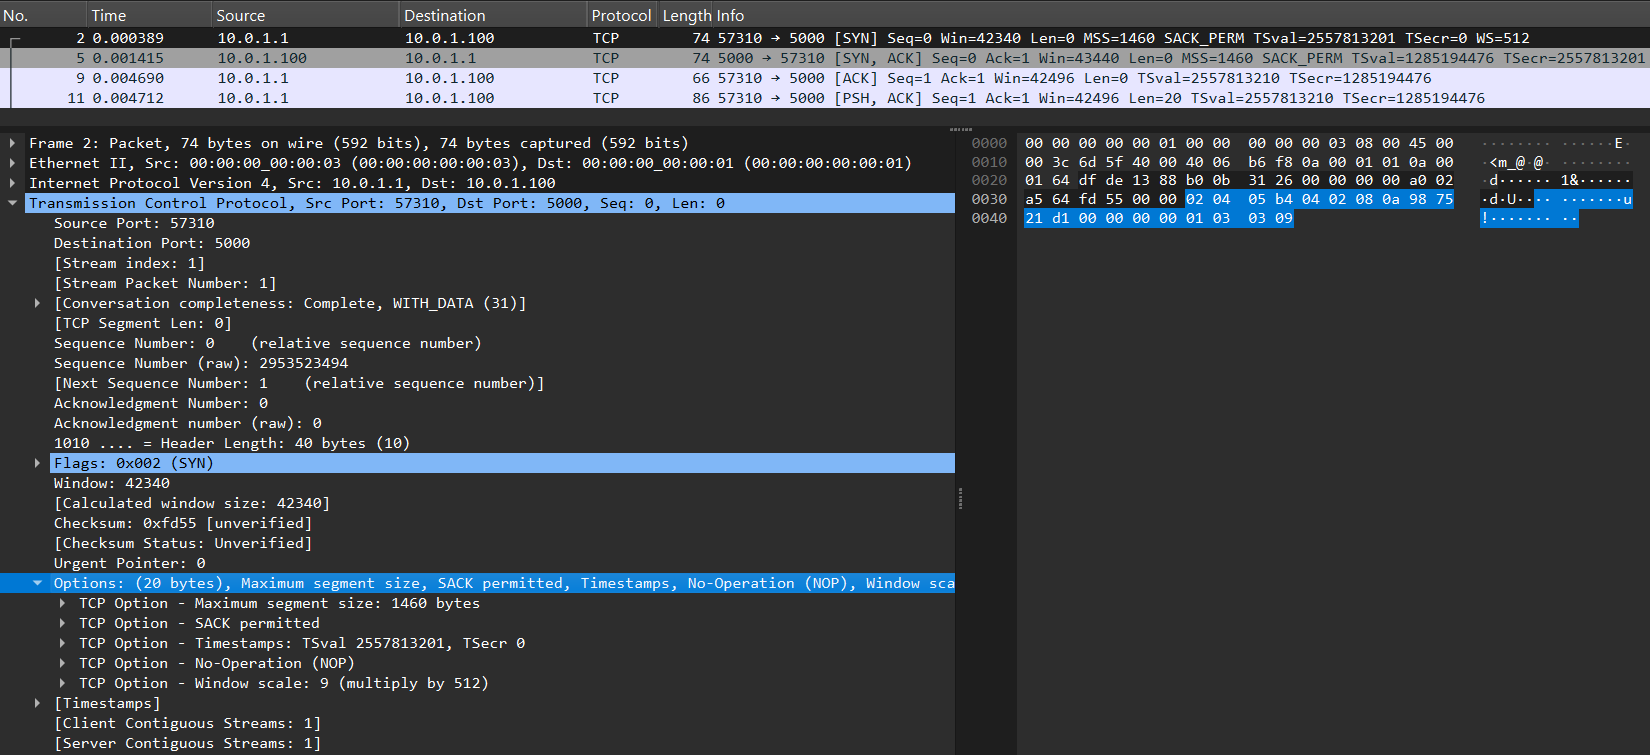
\includegraphics[width=\textwidth]{Images/ws_syn.png}
    \caption{Bắt tay ba bước giữa h1 và Edge Aggregator (K1, gói SYN số 2)}
    \label{fig:ws-syn}
\end{figure}
Gói SYN của \texttt{h1} mang MSS 1460, SACK permitted, Timestamps và Window scale 9 (nhân 512). SYN-ACK của Aggregator được gửi lại sau khoảng 1~ms, với cùng các tuỳ chọn. Gói số 11 là thông điệp HELLO dài 20 byte, gửi ngay sau ACK của bắt tay.

\begin{figure}[H]
    \centering
    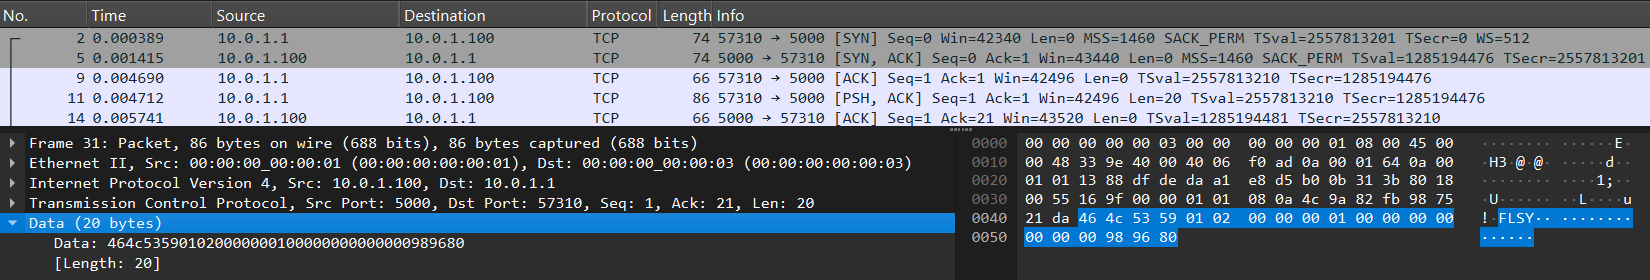
\includegraphics[width=\textwidth]{Images/ws_hdr.png}
    \caption{Header FLSync của thông điệp GLOBAL vòng 1 gửi tới h1 (K1, gói số 31)}
    \label{fig:ws-hdr}
\end{figure}
Vì \texttt{TCP\_NODELAY} được bật và header được gửi bằng một lời gọi \texttt{sendall()} riêng, 20 byte header đi trong một đoạn TCP riêng: \texttt{46 4C 53 59} (magic), \texttt{01} (version), \texttt{02} (GLOBAL), \texttt{00 00 00 01} (vòng 1), \texttt{00 00} (node 0, tức server), \texttt{00 00 00 00 00 98 96 80} (length $= 10\,000\,000$). Các đoạn tải tin sau đó đều dài 1448 byte (19\,472 trên 19\,486 đoạn có dữ liệu trong 30\,000 gói đầu của file).

\begin{figure}[H]
    \centering
    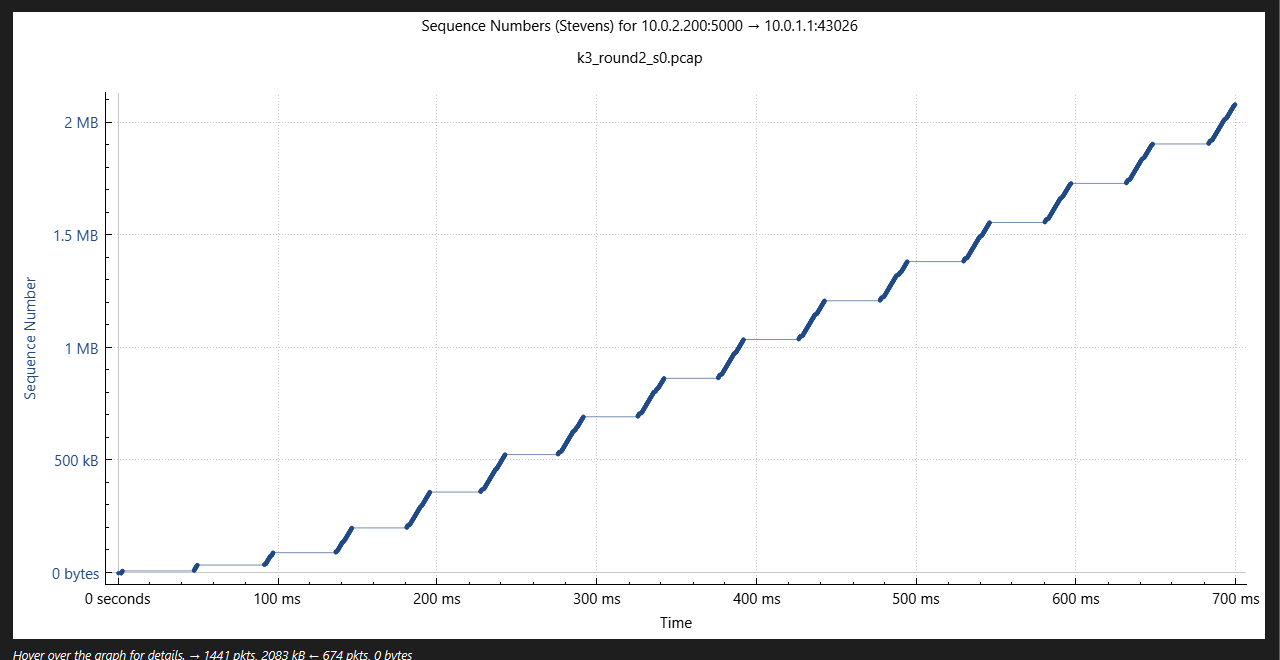
\includegraphics[width=\textwidth]{Images/ws_stevens.png}
    \caption{Biểu đồ Stevens của luồng cloud $\rightarrow$ h1 trong 0{,}7~s đầu vòng 2 (K3, WAN 100 Mbps, $N = 4$)}
    \label{fig:ws-stevens}
\end{figure}

\begin{figure}[H]
    \centering
    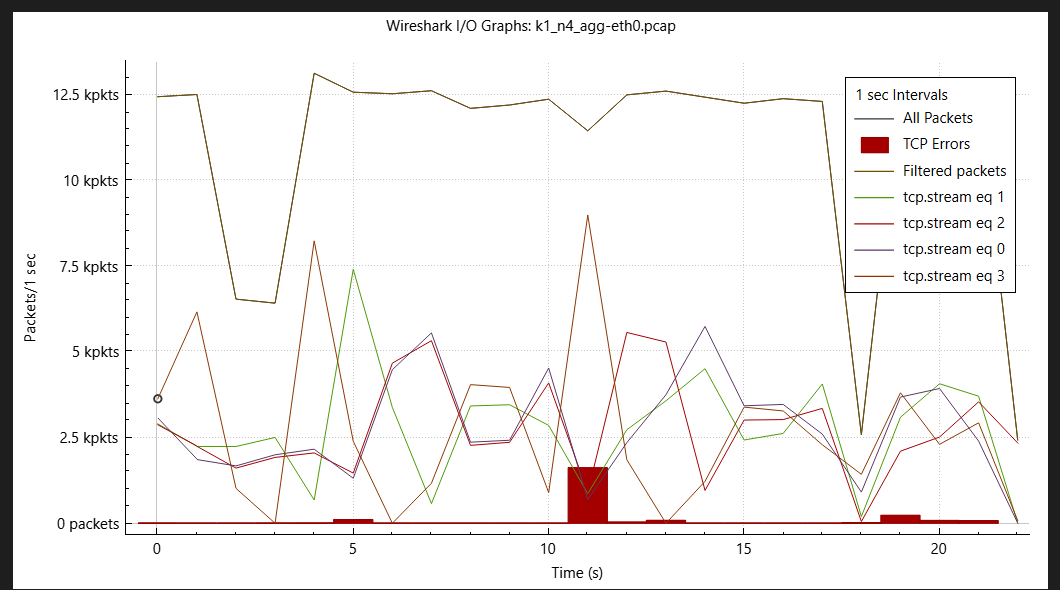
\includegraphics[width=0.9\textwidth]{Images/ws_io.png}
    \caption{I/O Graph của bốn luồng cùng chia link tới Aggregator (K1, $N = 4$, khoảng 1~s)}
    \label{fig:ws-io}
\end{figure}

\begin{figure}[H]
    \centering
    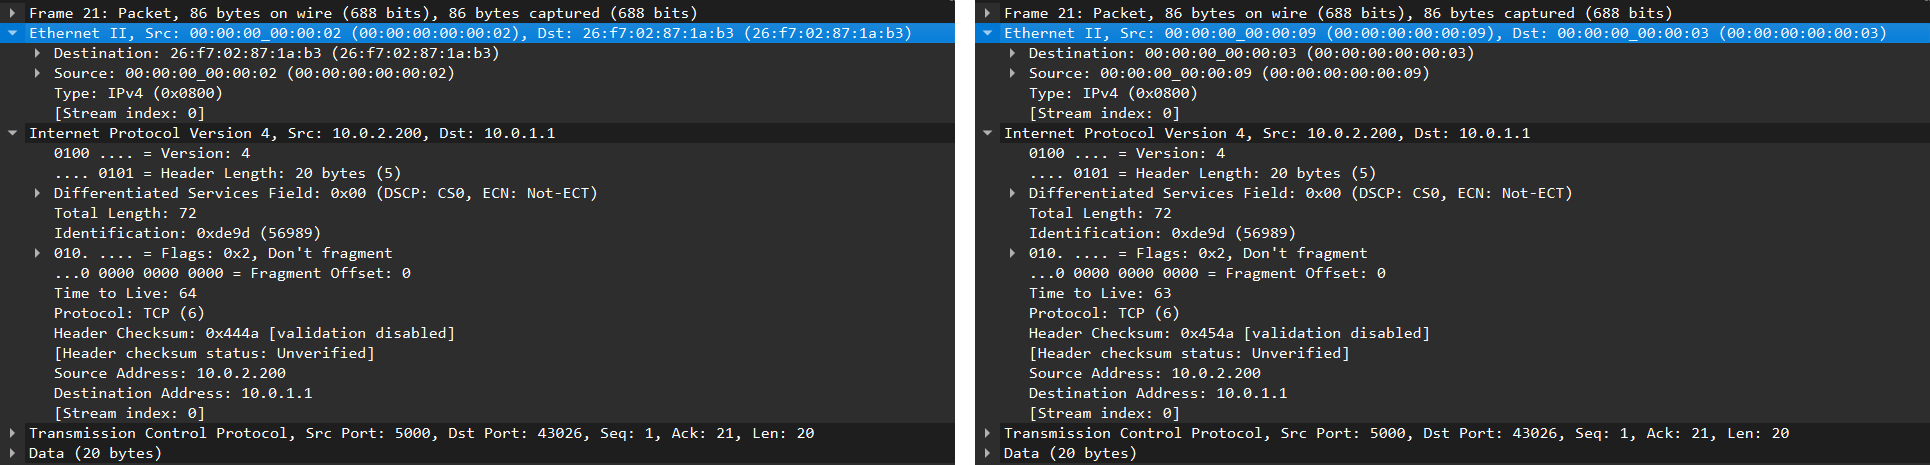
\includegraphics[width=\textwidth]{Images/ws_router.png}
    \caption{Cùng một gói trước (r1-eth1, trái) và sau (r1-eth0, phải) khi đi qua Edge Gateway r1}
    \label{fig:ws-router}
\end{figure}
Hai bản bắt có cùng Identification \texttt{0xde9d}, cùng địa chỉ IP nguồn và đích. Router giảm TTL từ 64 xuống 63, tính lại Header Checksum (\texttt{0x444a} thành \texttt{0x454a}), và thay cả hai địa chỉ MAC: trên mạng cloud khung đi từ \texttt{cloud} (\texttt{00:00:00:00:00:02}) tới \texttt{r1-eth1}; trên mạng biên khung đi từ \texttt{r1-eth0} (\texttt{00:00:00:00:00:09}) tới \texttt{h1} (\texttt{00:00:00:00:00:03}).

\subsection{Kết luận chương}
Topo gồm một nhánh biên RTT 4~ms và một nhánh WAN RTT 44~ms đi qua Edge Gateway \texttt{r1} (router kiêm firewall), cùng băng thông 100 Mbps, cho phép tách riêng ảnh hưởng của RTT. Giao thức FLSync giữ một kết nối TCP mỗi Edge Node, có ACK tầng ứng dụng để đo chính xác từng pha. Header các tầng tốn khoảng 4{,}6\% băng thông. Slow start lặp lại ở mọi vòng vì khoảng nghỉ huấn luyện 1~s dài hơn RTO.

\cleardoublepage

    \chaptercustom{4}{MÔ HÌNH GIẢI TÍCH VÀ KỊCH BẢN ĐO}
\setcounter{section}{4}
\setcounter{equation}{0}
Trước khi đo, nhóm xây dựng một mô hình giải tích đơn giản để dự đoán thời gian mỗi pha của vòng đồng bộ. Mô hình có hai tác dụng: cho biết trước kết quả ``đúng'' nên trông như thế nào để phát hiện lỗi cấu hình khi đo, và giúp giải thích phần chênh giữa số đo với lý thuyết. Chương này trình bày mô hình, các kịch bản đo và quy trình thu thập số liệu.

\subsection{Mô hình thời gian một pha truyền}
Xét $N$ luồng TCP song song, mỗi luồng truyền $S$ byte qua một link nghẽn chung có băng thông $B$, RTT cơ sở $R$. Giả thiết:
\begin{itemize}
    \item mỗi luồng bắt đầu slow start từ $IW = 10 \times 1448 = 14\,480$ byte (kết nối mới, hoặc sau khoảng nghỉ dài hơn RTO);
    \item tổng cửa sổ của $N$ luồng gấp đôi sau mỗi RTT cho tới khi đạt BDP, sau đó link được dùng hết ở tốc độ $\eta B$;
    \item không có mất gói ngoài lúc hàng đợi tràn, và các luồng chia đều băng thông.
\end{itemize}

Số RTT trong slow start và lượng dữ liệu đã gửi trong thời gian đó:
\begin{equation}
    k^{*} = \max\!\left(0,\ \left\lceil \log_2 \frac{B R / 8}{N \cdot IW} \right\rceil\right), \qquad
    D_{ss} = N \cdot IW \cdot \left(2^{k^{*}} - 1\right)
    \label{eq:ss}
\end{equation}

Nếu $D_{ss} < N S$, phần còn lại được truyền ở tốc độ đầy đủ:
\begin{equation}
    T_{phase}(N, S) = k^{*} R + \frac{8\,(N S - D_{ss})}{\eta B} + \frac{R}{2}
    \label{eq:tphase}
\end{equation}
Số hạng $R/2$ là thời gian để byte cuối cùng lan tới đích. Nếu khối đủ nhỏ để kết thúc ngay trong slow start ($D_{ss} \geq N S$), thời gian xấp xỉ $\lceil \log_2(S/IW + 1) \rceil R + R/2$.

Thời gian một vòng:
\begin{equation}
    T_{round} = T_{down} + T_{train} + T_{up} + T_{agg}
    \label{eq:tround}
\end{equation}
với $T_{down} = T_{phase}(N, S_{down})$, $T_{up} = T_{phase}(N, S_{up})$, $T_{train} = 1$~s và $T_{agg} \approx 0$.

Khi $N S$ lớn, số hạng thứ hai của~\eqref{eq:tphase} chiếm ưu thế và
\begin{equation}
    T_{phase} \approx \frac{8 N S}{\eta B}
    \label{eq:linear}
\end{equation}
tăng tuyến tính theo $N$ với hệ số góc $8S/(\eta B)$. Với $S = 10$~MB và $B = 100$~Mbps, hệ số góc là $0{,}837$~s cho mỗi Edge Node thêm vào, \emph{mỗi pha}.

Mô hình được cài đặt trong \texttt{code/model.py}; kết quả nằm trong thư mục \texttt{data/} dưới dạng các file \texttt{model\_<vị trí>\_<kích thước>.csv} và được dùng trực tiếp để vẽ biểu đồ ở Chương~5.

Mô hình không tính hành vi răng cưa của CUBIC sau mất gói, độ trễ hàng đợi làm RTT thực tế lớn hơn $R$, chi phí CPU của Mininet, và việc các luồng không bắt đầu đồng thời hoàn toàn. Vì vậy số đo được kỳ vọng lớn hơn mô hình một chút; nếu số đo nhỏ hơn mô hình đáng kể, nhiều khả năng cấu hình băng thông chưa có hiệu lực.

\subsection{Kịch bản đo}
Năm kịch bản trong Bảng~\ref{tab:scen} được cài sẵn trong \texttt{code/run\_experiments.py}; mỗi kịch bản chạy với $N = 2, 3, 4, 5, 6$.

\begin{table}[H]
    \centering
    \caption{Các kịch bản đo}
    \label{tab:scen}
    \begin{tabular}{l l c c c l}
        \toprule
        \textbf{Mã} & \textbf{Aggregator} & \textbf{WAN} & $S_{down}$ & $S_{up}$ & \textbf{Phục vụ} \\
        \midrule
        K1\_edge\_full & Edge & -- & 10 MB & 10 MB & Q1, Q2, Q3 \\
        K2\_edge\_comp & Edge & -- & 10 MB & 1 MB & Q2 \\
        K2\_cloud\_comp & Cloud & 100 Mbps & 10 MB & 1 MB & Q2 \\
        K3\_cloud\_full & Cloud & 100 Mbps & 10 MB & 10 MB & Q2, Q3 \\
        K3\_cloud20\_full & Cloud & 20 Mbps & 10 MB & 10 MB & Q3 \\
        \bottomrule
    \end{tabular}
\end{table}

Ở kịch bản nén, chỉ chiều lên được nén vì đây là cách các kỹ thuật nén gradient thường áp dụng: máy khách gửi gradient thưa, còn mô hình toàn cục phát xuống vẫn đầy đủ.

\subsection{Quy trình đo}
\begin{enumerate}
    \item Khởi tạo topo mới cho mỗi lần đo, tắt TSO/GSO/GRO trên mọi giao diện.
    \item Bật \texttt{ping -i 0.2} từ \texttt{h1} tới nút tổng hợp trong suốt lần đo để ghi RTT khi có tải.
    \item (Tuỳ chọn \texttt{-{}-pcap}) bật \texttt{tcpdump} trên giao diện của nút tổng hợp.
    \item Chạy \texttt{fl\_server.py} trên nút tổng hợp, sau đó $N$ tiến trình \texttt{fl\_client.py} trên \texttt{h1..hN}.
    \item Server ghi mỗi vòng một dòng gồm $T_{down}$, $T_{up}$, $T_{round}$ vào \texttt{results/<kịch bản>\_n<N>.csv}.
    \item Sau 10 vòng, dừng mọi tiến trình và huỷ topo.
    \item Chạy \texttt{code/summarize.py}: bỏ vòng 1 (ARP, bắt tay, khởi động Python), lấy trung bình và độ lệch chuẩn của 9 vòng còn lại, ghi vào \texttt{data/measured\_<kịch bản>.csv}.
\end{enumerate}

Lệnh chạy toàn bộ:
\codesnap{run_all}

\subsection{Cách đo từng chỉ số}
\begin{itemize}
    \item $T_{down}$: từ lúc server bắt đầu gửi \texttt{GLOBAL} tới lúc nhận \texttt{ACK} tầng ứng dụng của client cuối cùng.
    \item $T_{up}$: từ lúc client đầu tiên kết thúc huấn luyện tới lúc \texttt{UPDATE} cuối cùng tới server, tính bằng $\max(t_{update}) - \min(t_{ack}) - T_{train}$.
    \item $T_{round}$: từ lúc bắt đầu gửi \texttt{GLOBAL} tới lúc server gửi xong \texttt{ACK} kết thúc vòng.
    \item RTT khi có tải: giá trị \texttt{ping} trong khoảng thời gian có truyền dữ liệu, so với RTT lúc rảnh.
    \item $d_{trans}$ hiệu dụng: $T_{up}$ trừ phần slow start đọc từ biểu đồ Stevens.
\end{itemize}

\subsection{Các yếu tố ảnh hưởng độ tin cậy}
Mininet chạy mọi host trên cùng một nhân hệ điều hành, nên CPU của máy ảo là nguồn sai số lớn nhất. Nhóm cấp ít nhất 2 vCPU và chỉ đo khi \texttt{iperf} đạt gần 95 Mbps. Đồng hồ thì không gây sai số: mọi thời điểm đều lấy trên server.

Hai nguồn sai số còn lại nằm ở cách đo. Nếu lấy $T_{down}$ theo thời điểm \texttt{sendall()} trả về, kết quả sẽ nhỏ hơn thực tế vài trăm ms; ACK tầng ứng dụng của FLSync có để tránh lỗi này. Kích thước hàng đợi (\nolinkurl{max_queue_size}) cũng ảnh hưởng: quá lớn thì RTT khi có tải tăng mạnh, quá nhỏ thì mất gói liên tục. Nhóm chọn 200 gói, tức tối đa khoảng 24~ms trễ hàng đợi ở 100 Mbps.

\subsection{Kết luận chương}
Mô hình giải tích dự đoán thời gian mỗi pha tăng tuyến tính theo $N$ với hệ số góc khoảng 0{,}84~s mỗi Edge Node cho khối 10 MB trên link 100 Mbps, cộng thêm một phần cố định do slow start phụ thuộc RTT. Năm kịch bản đo được thiết kế để kiểm chứng từng câu hỏi Q1--Q3 với cùng một quy trình tự động.

\cleardoublepage

    \chaptercustom{5}{KẾT QUẢ VÀ ĐÁNH GIÁ}
\setcounter{section}{5}
\setcounter{equation}{0}
Chương này trình bày kết quả cho từng câu hỏi Q1--Q3. Với mỗi câu hỏi, giá trị dự đoán từ mô hình giải tích ở Chương~4 được đặt cạnh cột số đo trên Mininet.

\textbf{Nguồn gốc số liệu.} Giá trị ``Mô hình'' tính bằng \texttt{code/model.py}. Giá trị ``Đo'' lấy từ Mininet 2.3.0 chạy trên Ubuntu 22.04 (WSL2), bằng \texttt{run\_experiments.py} và \texttt{summarize.py}: mỗi điểm là trung bình của 9 vòng (bỏ vòng 1), độ lệch chuẩn tính trên chính 9 vòng đó.

Cần lưu ý cách server ghi thời gian (\texttt{fl\_server.py}): $T_{down}$ tính tới khi Edge Node \emph{cuối cùng} nhận xong mô hình, còn $T_{up}$ tính từ lúc Edge Node \emph{đầu tiên} train xong. Nếu các luồng tải xuống không kết thúc cùng lúc, nút xong sớm bắt đầu upload trong khi nút khác còn đang tải xuống; hai pha chồng lên nhau, nên số đo $T_{round}$ có thể nhỏ hơn $T_{down} + T_{train} + T_{up}$, và $T_{up}$ đo được bao gồm cả độ lệch thời điểm kết thúc tải xuống giữa các nút.

\subsection{Kiểm tra môi trường}
Trước khi đo, nhóm dựng topo bằng \texttt{tools/sanity.py} (giống \texttt{topo.py}, thêm bước tắt TSO/GSO/GRO như \texttt{run\_experiments.py}) rồi chạy ping và iperf trong Mininet CLI. Hình~\ref{fig:sanity100} và Hình~\ref{fig:sanity20} là ảnh chụp terminal của hai lần chạy, với WAN 100 Mbps và 20 Mbps.

\begin{figure}[H]
    \centering
    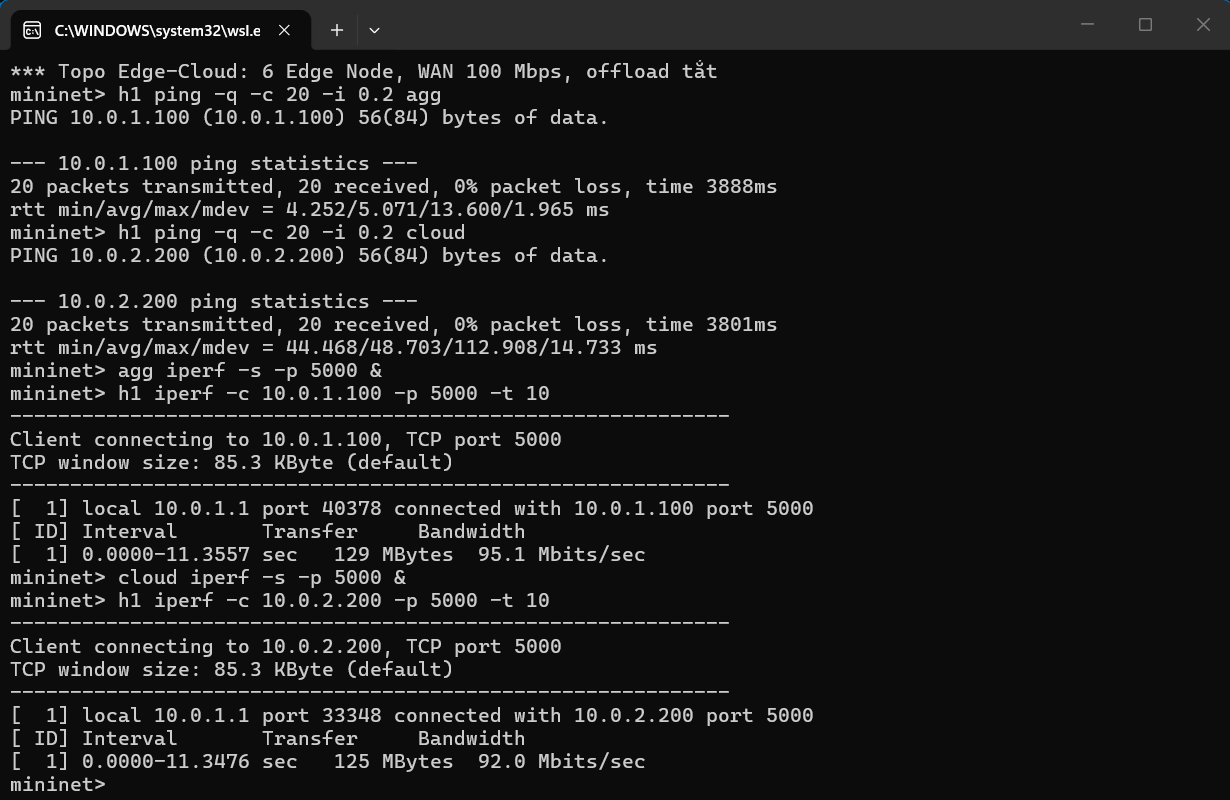
\includegraphics[width=0.85\textwidth]{Images/run/sanity_wan100.png}
    \caption{Kiểm tra RTT và thông lượng trong Mininet CLI, WAN 100 Mbps}
    \label{fig:sanity100}
\end{figure}

\begin{figure}[H]
    \centering
    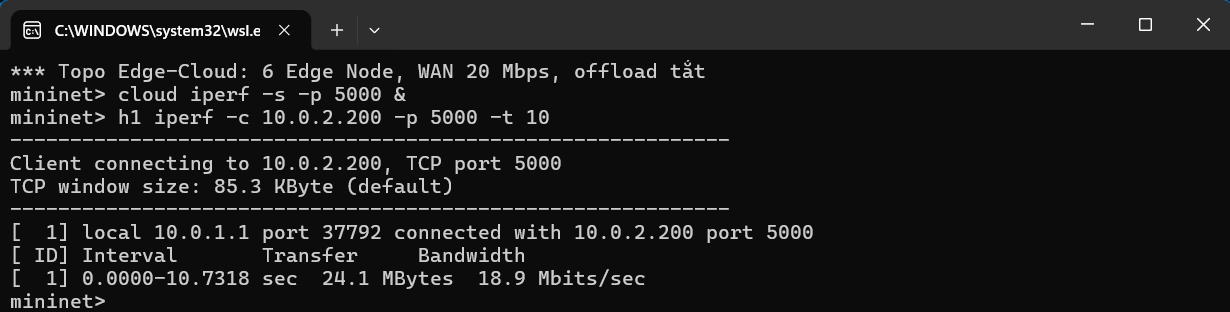
\includegraphics[width=0.85\textwidth]{Images/run/sanity_wan20.png}
    \caption{Kiểm tra thông lượng tới Cloud Server, WAN 20 Mbps}
    \label{fig:sanity20}
\end{figure}

RTT đo bằng 20 gói \texttt{ping} cách nhau 0{,}2~s; \texttt{iperf} chạy 10~s trên cổng 5000, cổng duy nhất firewall của \texttt{r1} cho phép tới Cloud Server. RTT nhỏ nhất là 4{,}25~ms tới \texttt{agg} và 44{,}47~ms tới \texttt{cloud}, khớp với giá trị kỳ vọng 4 và 44~ms. RTT trung bình (5{,}07 và 48{,}70~ms) cao hơn vì gói đầu tiên phải chờ phân giải ARP (13{,}6 và 112{,}9~ms). Thông lượng iperf là 95{,}1 Mbps tới \texttt{agg}, 92{,}0 Mbps tới \texttt{cloud} qua WAN 100 Mbps và 18{,}9 Mbps qua WAN 20 Mbps, đều không thấp hơn quá 4\% so với giới hạn $\eta B$ (95{,}6 và 19{,}1 Mbps). Cấu hình băng thông và độ trễ của topo vì vậy có hiệu lực.

Hình~\ref{fig:runk1} là ảnh chụp một lần chạy thử kịch bản K1 với $N = 4$ và 5 vòng, gõ trực tiếp trong Mininet CLI: bốn Edge Node chạy nền, Aggregator in thời gian từng vòng rồi ghi log CSV. $T_{round}$ của vòng 2--5 là 7{,}27--7{,}46~s, khớp với giá trị trung bình 7{,}333~s ở Bảng~\ref{tab:q1}.

\begin{figure}[H]
    \centering
    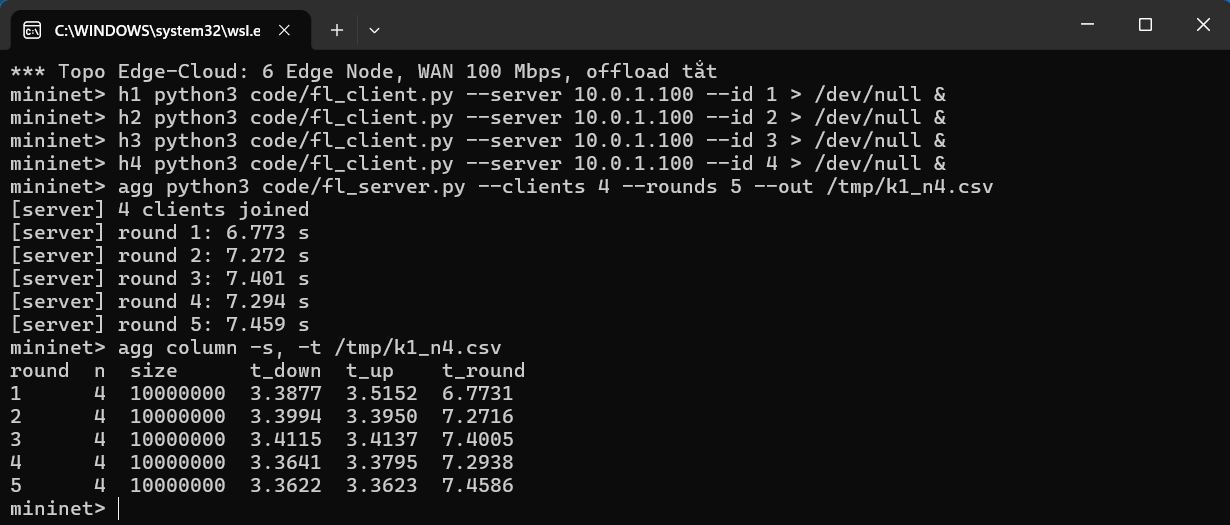
\includegraphics[width=0.85\textwidth]{Images/run/run_k1_n4.png}
    \caption{Một lần chạy kịch bản K1, $N = 4$, 5 vòng: log của Aggregator và file CSV}
    \label{fig:runk1}
\end{figure}

\subsection{Q1 -- Ảnh hưởng của số Edge Node}
Bảng~\ref{tab:q1} và Hình~\ref{fig:q1} cho thời gian các pha của kịch bản K1 (Aggregator tại biên, 10 MB mỗi chiều).

\begin{table}[H]
    \centering
    \caption{Thời gian các pha theo số Edge Node, kịch bản K1 (giây)}
    \label{tab:q1}
    \begin{tabular}{c c c c c c}
        \toprule
        \multirow{2}{*}{$N$} & \multicolumn{3}{c}{\textbf{Mô hình}} & \multicolumn{2}{c}{\textbf{Đo}} \\
        \cmidrule(lr){2-4} \cmidrule(lr){5-6}
        & $T_{down}$ & $T_{up}$ & $T_{round}$ & $T_{round}$ & độ lệch chuẩn \\
        \midrule
        2 & 1,677 & 1,677 & 4,353 & 4,446 & 0,036 \\
        3 & 2,512 & 2,512 & 6,024 & 5,882 & 0,114 \\
        4 & 3,348 & 3,348 & 7,696 & 7,333 & 0,117 \\
        5 & 4,184 & 4,184 & 9,369 & 8,566 & 0,207 \\
        6 & 5,021 & 5,021 & 11,042 & 9,943 & 0,311 \\
        \bottomrule
    \end{tabular}
\end{table}

\begin{figure}[H]
    \centering
    \begin{tikzpicture}
        \begin{axis}[
            width=0.85\textwidth, height=7cm,
            xlabel={Số Edge Node $N$}, ylabel={Thời gian (s)},
            xmin=1.8, xmax=6.2, xtick={2,3,4,5,6},
            ymin=0, grid=major, grid style={gray!25},
            legend pos=north west, legend cell align=left,
            restrict x to domain=2:6,
        ]
            \addplot[thick, blue, mark=*] table[x=n, y=t_round, col sep=comma] {data/model_edge_10MB.csv};
            \addlegendentry{$T_{round}$ (mô hình)}
            \addplot[thick, blue!50, mark=square, dashed] table[x=n, y=t_up, col sep=comma] {data/model_edge_10MB.csv};
            \addlegendentry{$T_{up}$ (mô hình)}
            \addplot[red, mark=triangle*, error bars/.cd, y dir=both, y explicit]
                table[x=n, y=t_round, y error=t_round_sd, col sep=comma] {data/measured_K1_edge_full.csv};
            \addlegendentry{$T_{round}$ (đo)}
        \end{axis}
    \end{tikzpicture}
    \caption{Thời gian một vòng theo số Edge Node, Aggregator tại biên, 10 MB}
    \label{fig:q1}
\end{figure}

\textbf{Nhận xét.} Theo mô hình, mỗi Edge Node thêm vào làm mỗi pha dài thêm khoảng 0{,}84~s, tức $T_{round}$ tăng khoảng 1{,}67~s. Từ $N = 2$ lên $N = 6$, $T_{round}$ tăng từ 4{,}35~s lên 11{,}04~s (gấp 2{,}5 lần), trong khi phần huấn luyện cố định 1~s không đổi. Nguyên nhân là link 100 Mbps tới Aggregator đã bão hoà ngay từ $N = 1$: thêm Edge Node không làm tổng thông lượng tăng mà chỉ chia nhỏ phần của mỗi nút ($B/N$, còn khoảng 16 Mbps mỗi nút khi $N = 6$). Trong khi đó, mỗi link truy nhập của Edge Node có 100 Mbps nhưng chỉ dùng được $1/N$.

Bảng~\ref{tab:q1thr} cho thông lượng của pha upload, tính bằng $8NS/T_{up}$. Thông lượng gộp đứng yên ở khoảng 95{,}6 Mbps (giới hạn $\eta B$ của link 100 Mbps), còn phần của mỗi nút giảm theo $1/N$.

\begin{table}[H]
    \centering
    \caption{Thông lượng ứng dụng của pha upload, kịch bản K1 (Mbps)}
    \label{tab:q1thr}
    \begin{tabular}{c c c c c}
        \toprule
        \multirow{2}{*}{$N$} & \multicolumn{2}{c}{\textbf{Mô hình}} & \multicolumn{2}{c}{\textbf{Đo}} \\
        \cmidrule(lr){2-3} \cmidrule(lr){4-5}
        & gộp & mỗi nút & gộp & mỗi nút \\
        \midrule
        2 & 95,4 & 47,7 & 91,2 & 45,6 \\
        3 & 95,6 & 31,9 & 93,1 & 31,0 \\
        4 & 95,6 & 23,9 & 94,8 & 23,7 \\
        5 & 95,6 & 19,1 & 94,4 & 18,9 \\
        6 & 95,6 & 15,9 & 92,1 & 15,4 \\
        \bottomrule
    \end{tabular}
\end{table}

Cột ``Đo'' lấy từ cột \texttt{thr\_mbps} do \texttt{summarize.py} tính, và có thể đối chiếu với \emph{Statistics $\rightarrow$ Conversations} trên Wireshark. Link nghẽn vì vậy là link \texttt{s1}--\texttt{agg}, tức \emph{giao diện mạng của nút tổng hợp}; link truy nhập của mỗi Edge Node còn dư $(N-1)/N$ băng thông. Muốn rút ngắn vòng khi tăng số nút, phải tăng băng thông vào Aggregator, giảm kích thước dữ liệu (Q2), hoặc chia tải cho nhiều Aggregator (tổng hợp phân cấp).

\textbf{Đối chiếu với số đo.} (1) Thông lượng gộp đo được 91--95 Mbps ở mọi $N$, khớp với nhận định link \texttt{s1}--\texttt{agg} bão hoà. (2) $T_{down}$ đo tăng từ 1{,}717~s ($N = 2$) lên 5{,}159~s ($N = 6$), tức khoảng 0{,}86~s mỗi nút, gần với hệ số góc 0{,}84~s của mô hình. (3) Tuy vậy $T_{round}$ đo chỉ tăng khoảng 1{,}37~s mỗi nút (thay vì 1{,}67~s) và từ $N = 3$ trở đi nhỏ hơn mô hình, tới 1{,}1~s ở $N = 6$ (9{,}94~s so với 11{,}04~s). Nguyên nhân là các pha chồng lên nhau: nút nhận xong mô hình sớm bắt đầu upload trong khi nút khác còn tải xuống, nên $T_{round}$ nhỏ hơn $T_{down} + 1 + T_{up} = 11{,}37$~s; mô hình giả thiết các pha nối tiếp nhau. (4) Độ lệch chuẩn tăng từ 0{,}036~s lên 0{,}311~s khi $N$ tăng, cho thấy các luồng chia băng thông kém đều hơn khi có nhiều nút.

\subsection{Q2 -- Gửi toàn bộ mô hình so với gradient nén}
Câu hỏi Q2 được xét trên ba chỉ số: thời gian pha upload, thời gian cả vòng và RTT khi có tải.

\subsubsection{Thời gian truyền chiều lên}
Bảng~\ref{tab:q2} so sánh $T_{up}$ khi gửi 10 MB và 1 MB, ở cả hai vị trí Aggregator.

\begin{table}[H]
    \centering
    \caption{Thời gian pha upload $T_{up}$ (giây) và hệ số giảm khi nén 1/10, giá trị mô hình}
    \label{tab:q2}
    \begin{tabular}{c c c c c c c}
        \toprule
        \multirow{2}{*}{$N$} & \multicolumn{3}{c}{\textbf{Edge (RTT 4 ms)}} & \multicolumn{3}{c}{\textbf{Cloud (RTT 44 ms, 100 Mbps)}} \\
        \cmidrule(lr){2-4} \cmidrule(lr){5-7}
        & 10 MB & 1 MB & giảm & 10 MB & 1 MB & giảm \\
        \midrule
        1 & 0,843 & 0,090 & 9,4$\times$ & 1,046 & 0,293 & 3,6$\times$ \\
        2 & 1,677 & 0,171 & 9,8$\times$ & 1,840 & 0,334 & 5,5$\times$ \\
        3 & 2,512 & 0,253 & 9,9$\times$ & 2,653 & 0,394 & 6,7$\times$ \\
        4 & 3,348 & 0,337 & 9,9$\times$ & 3,471 & 0,460 & 7,5$\times$ \\
        5 & 4,184 & 0,420 & 10,0$\times$ & 4,294 & 0,530 & 8,1$\times$ \\
        6 & 5,021 & 0,504 & 10,0$\times$ & 5,122 & 0,605 & 8,5$\times$ \\
        \bottomrule
    \end{tabular}
\end{table}

\begin{figure}[H]
    \centering
    \begin{tikzpicture}
        \begin{axis}[
            width=0.85\textwidth, height=7cm,
            xlabel={Số Edge Node $N$}, ylabel={$T_{up}$ (s)},
            xmin=0.8, xmax=6.2, xtick={1,...,6},
            ymode=log, log basis y=10,
            grid=major, grid style={gray!25},
            legend style={at={(0.5,-0.3)}, anchor=north, legend columns=2}, legend cell align=left,
        ]
            \addplot[thick, blue, mark=*] table[x=n, y=t_up, col sep=comma] {data/model_edge_10MB.csv};
            \addlegendentry{Edge, 10 MB}
            \addplot[thick, blue, mark=o, dashed] table[x=n, y=t_up, col sep=comma] {data/model_edge_1MB.csv};
            \addlegendentry{Edge, 1 MB}
            \addplot[thick, orange, mark=square*] table[x=n, y=t_up, col sep=comma] {data/model_cloud_10MB.csv};
            \addlegendentry{Cloud, 10 MB}
            \addplot[thick, orange, mark=square, dashed] table[x=n, y=t_up, col sep=comma] {data/model_cloud_1MB.csv};
            \addlegendentry{Cloud, 1 MB}
            \addplot[red, mark=triangle*] table[x=n, y=t_up, col sep=comma] {data/measured_K2_edge_comp.csv};
            \addlegendentry{Edge, 1 MB (đo)}
            \addplot[red!60!black, mark=diamond*] table[x=n, y=t_up, col sep=comma] {data/measured_K2_cloud_comp.csv};
            \addlegendentry{Cloud, 1 MB (đo)}
        \end{axis}
    \end{tikzpicture}
    \caption{Thời gian upload khi gửi toàn bộ mô hình và gradient nén (trục tung logarit)}
    \label{fig:q2}
\end{figure}

\textbf{Nhận xét.} Ở biên, nén 1/10 giảm $T_{up}$ gần đúng 10 lần, vì RTT chỉ 4~ms và slow start kết thúc sau 2 RTT; gần như toàn bộ thời gian là $d_{trans}$, tỷ lệ thuận với kích thước.

Qua WAN, mức giảm thấp hơn nhiều khi ít nút: chỉ 3{,}6 lần với $N = 1$. Một luồng gửi 1 MB phải qua khoảng 6 RTT slow start (264~ms) trước khi cửa sổ đủ lớn, trong khi $d_{trans}$ của 1 MB ở 100 Mbps chỉ khoảng 84~ms. Nén làm giảm $d_{trans}$ nhưng không giảm được số RTT. Khi $N$ tăng, tổng cửa sổ của $N$ luồng lấp đầy BDP nhanh hơn ($k^{*}$ nhỏ đi) và $d_{trans}$ lại chiếm ưu thế, nên mức giảm tiến dần về 10 lần.

Với thiết kế hệ thống, điều này có nghĩa là nén gradient có lợi nhất khi link chậm hoặc nhiều nút cùng chia link. Với ít nút qua WAN có RTT lớn, cần kết hợp thêm biện pháp ở tầng giao vận, ví dụ tắt \nolinkurl{tcp_slow_start_after_idle} để giữ $cwnd$ giữa các vòng, hoặc tăng IW.

Bảng~\ref{tab:q2meas} cho $T_{up}$ đo được của bốn kịch bản (K1, K2\_edge, K3\_cloud, K2\_cloud).

\begin{table}[H]
    \centering
    \caption{Thời gian pha upload $T_{up}$ (giây) và hệ số giảm khi nén 1/10, số đo}
    \label{tab:q2meas}
    \begin{tabular}{c c c c c c c}
        \toprule
        \multirow{2}{*}{$N$} & \multicolumn{3}{c}{\textbf{Edge}} & \multicolumn{3}{c}{\textbf{Cloud (100 Mbps)}} \\
        \cmidrule(lr){2-4} \cmidrule(lr){5-7}
        & 10 MB & 1 MB & giảm & 10 MB & 1 MB & giảm \\
        \midrule
        2 & 1,755 & 0,259 & 6,8$\times$ & 2,733 & 0,798 & 3,4$\times$ \\
        3 & 2,578 & 0,333 & 7,7$\times$ & 3,321 & 1,762 & 1,9$\times$ \\
        4 & 3,374 & 0,481 & 7,0$\times$ & 4,975 & 1,518 & 3,3$\times$ \\
        5 & 4,235 & 0,901 & 4,7$\times$ & 6,911 & 2,419 & 2,9$\times$ \\
        6 & 5,214 & 1,424 & 3,7$\times$ & 7,112 & 3,117 & 2,3$\times$ \\
        \bottomrule
    \end{tabular}
\end{table}

Số đo cho mức giảm thấp hơn mô hình, và khác mô hình ở chỗ mức giảm \emph{giảm dần} khi $N$ tăng (Edge: từ 6{,}8 xuống 3{,}7 lần). Lý do nằm ở cách đo đã nêu đầu chương: $T_{up}$ tính từ lúc nút đầu tiên train xong, nên bao gồm khoảng lệch giữa nút nhận xong mô hình 10 MB sớm nhất và muộn nhất. Khoảng lệch này không phụ thuộc kích thước bản cập nhật và tăng theo $N$; khi bản cập nhật chỉ còn 1 MB, nó chiếm phần lớn $T_{up}$. Qua WAN, sự chênh lệch giữa các luồng còn lớn hơn (độ lệch chuẩn tới 0{,}65~s ở K2\_cloud), nên mức giảm chỉ còn 1{,}9--3{,}4 lần. Nói cách khác, khi chiều lên đã được nén, sự không đều của pha tải xuống trở thành yếu tố quyết định thời gian chờ của Aggregator.

\subsubsection{Thời gian vòng khi chỉ nén chiều lên}
Vì mô hình toàn cục phát xuống vẫn là 10 MB, lợi ích trên toàn vòng nhỏ hơn lợi ích trên pha upload. Với $N = 6$ tại biên, $T_{round}$ giảm từ 11{,}04~s xuống $5{,}02 + 1 + 0{,}50 = 6{,}53$~s (giảm 41\%); tại Cloud 100 Mbps, từ 11{,}24~s xuống 6{,}73~s. Pha phát xuống trở thành phần chiếm ưu thế, gợi ý rằng bước tiếp theo nên là nén cả chiều xuống hoặc dùng multicast.

Số đo với $N = 6$: tại biên $T_{round}$ giảm từ 9{,}94~s (K1) xuống 6{,}17~s (K2\_edge), tức giảm 38\%; tại Cloud 100 Mbps giảm từ 11{,}80~s (K3\_cloud) xuống 7{,}52~s (K2\_cloud), tức giảm 36\%. Mức giảm trên toàn vòng gần với dự đoán của mô hình (41\% và 40\%), dù mức giảm của riêng pha upload thấp hơn nhiều.

\subsubsection{RTT khi có tải}
Trong lúc $N$ luồng cùng đẩy dữ liệu, hàng đợi tại cổng \texttt{s1} hướng tới Aggregator đầy dần. Với hàng đợi 200 gói, công thức~\eqref{eq:dqueue} ở Chương~2 cho độ trễ hàng đợi tối đa khoảng 24~ms, nên RTT đo bằng ping từ \texttt{h1} có thể tăng từ 4~ms lên gần 28~ms trong pha upload. Khi nén 1/10, thời gian hàng đợi bị đầy rút ngắn khoảng 10 lần, và với ít nút các luồng 1 MB có thể kết thúc trước khi hàng đợi kịp đầy. Bảng~\ref{tab:q2rtt} cho số đo.

\begin{table}[H]
    \centering
    \caption{RTT từ h1 tới Aggregator trong suốt lần đo, $N = 6$ (ms)}
    \label{tab:q2rtt}
    \begin{tabular}{l c c c}
        \toprule
        \textbf{Kịch bản} & \textbf{RTT rảnh} & \textbf{RTT trung bình khi có tải} & \textbf{RTT lớn nhất} \\
        \midrule
        Edge, 10 MB (K1) & 4,3 & 32,2 & 58,5 \\
        Edge, 1 MB (K2) & 4,3 & 35,9 & 54,1 \\
        Cloud, 10 MB (K3) & 44,5 & 62,0 & 95,3 \\
        Cloud, 1 MB (K2) & 44,5 & 63,3 & 92,9 \\
        \bottomrule
    \end{tabular}
\end{table}

RTT rảnh là RTT nhỏ nhất ở Hình~\ref{fig:sanity100}, không tính gói đầu chờ ARP. RTT khi có tải tính trên toàn bộ log \texttt{ping -i 0.2} của lần đo, gồm cả pha tải xuống và pha upload, vì log không ghi mốc thời gian để tách riêng từng pha.

RTT lớn nhất đo được (54--58~ms tại biên) vượt mức khoảng 28~ms dự đoán cho riêng hàng đợi chiều lên. Do các pha chồng lên nhau, có lúc hàng đợi 200 gói ở cả hai chiều của link \texttt{s1}--\texttt{agg} cùng đầy; $4 + 24 + 24 \approx 52$~ms, gần với giá trị đo. Nén chiều lên không làm giảm RTT trung bình (35{,}9~ms so với 32{,}2~ms tại biên), vì pha tải xuống 10 MB vẫn làm đầy hàng đợi chiều xuống trong phần lớn thời gian của vòng.

\subsection{Q3 -- Tổng hợp tại Edge so với tại Cloud}
\begin{figure}[H]
    \centering
    \begin{tikzpicture}
        \begin{axis}[
            width=0.85\textwidth, height=7cm,
            xlabel={Số Edge Node $N$}, ylabel={$T_{round}$ (s)},
            xmin=1.8, xmax=6.2, xtick={2,3,4,5,6},
            ymin=0, grid=major, grid style={gray!25},
            legend pos=north west, legend cell align=left,
            restrict x to domain=2:6,
        ]
            \addplot[thick, blue, mark=*] table[x=n, y=t_round, col sep=comma] {data/model_edge_10MB.csv};
            \addlegendentry{Edge (RTT 4 ms, 100 Mbps)}
            \addplot[thick, orange, mark=square*] table[x=n, y=t_round, col sep=comma] {data/model_cloud_10MB.csv};
            \addlegendentry{Cloud (RTT 44 ms, 100 Mbps)}
            \addplot[thick, red!70!black, mark=triangle*] table[x=n, y=t_round, col sep=comma] {data/model_cloud20_10MB.csv};
            \addlegendentry{Cloud (RTT 44 ms, 20 Mbps)}
            \addplot[blue, only marks, mark=x, mark size=4pt, forget plot] table[x=n, y=t_round, col sep=comma] {data/measured_K1_edge_full.csv};
            \addplot[orange, only marks, mark=x, mark size=4pt, forget plot] table[x=n, y=t_round, col sep=comma] {data/measured_K3_cloud_full.csv};
            \addplot[red!70!black, only marks, mark=x, mark size=4pt] table[x=n, y=t_round, col sep=comma] {data/measured_K3_cloud20_full.csv};
            \addlegendentry{Số đo (dấu $\times$, cùng màu)}
        \end{axis}
    \end{tikzpicture}
    \caption{Thời gian một vòng theo vị trí Aggregator, 10 MB mỗi chiều}
    \label{fig:q3}
\end{figure}

\begin{table}[H]
    \centering
    \caption{$T_{round}$ theo vị trí Aggregator (giây), giá trị mô hình và số đo}
    \label{tab:q3}
    \resizebox{\textwidth}{!}{%
    \begin{tabular}{c c c c c c c c c}
        \toprule
        \multirow{2}{*}{$N$} & \multicolumn{4}{c}{\textbf{Mô hình}} & \multicolumn{4}{c}{\textbf{Đo}} \\
        \cmidrule(lr){2-5} \cmidrule(lr){6-9}
        & Edge & Cloud 100M & chênh & Cloud 20M & Edge & Cloud 100M & chênh & Cloud 20M \\
        \midrule
        2 & 4,353 & 4,680 & 0,327 & 17,877 & 4,446 & 5,480 & 1,034 & 17,540 \\
        3 & 6,024 & 6,306 & 0,282 & 26,205 & 5,882 & 6,312 & 0,430 & 25,035 \\
        4 & 7,696 & 7,942 & 0,247 & 34,542 & 7,333 & 8,361 & 1,028 & 33,137 \\
        5 & 9,369 & 9,588 & 0,219 & 42,895 & 8,566 & 10,090 & 1,524 & 40,457 \\
        6 & 11,042 & 11,244 & 0,202 & 51,247 & 9,943 & 11,803 & 1,860 & 48,382 \\
        \bottomrule
    \end{tabular}}
\end{table}

\textbf{Nhận xét.} Khi băng thông WAN bằng băng thông nhánh biên, chênh lệch giữa Cloud và Edge chỉ còn 0{,}2--0{,}33~s mỗi vòng, tức 2--7\% $T_{round}$. Phần chênh này đến từ hai nguồn: slow start dài hơn (6 RTT $\times$ 44~ms thay vì 2 RTT $\times$ 4~ms, xảy ra ở cả hai pha) và thêm nửa RTT lan truyền cho mỗi pha. Bắt tay chỉ xảy ra một lần khi kết nối nên không góp vào các vòng sau. Chênh lệch giảm dần khi $N$ tăng vì tổng cửa sổ của nhiều luồng lấp đầy BDP sau ít RTT hơn.

Khi WAN chỉ có 20 Mbps, $T_{round}$ gấp khoảng 4{,}6 lần so với Edge ở $N = 6$ (51{,}2~s so với 11{,}0~s). Phần chênh do RTT (khoảng 0{,}2~s) lúc này nhỏ hơn 1\% so với phần chênh do băng thông.

\textbf{Đối chiếu với số đo.} Với WAN 20 Mbps, số đo bám sát mô hình (sai khác dưới 6\%), và Cloud chậm hơn Edge 4{,}9 lần ở $N = 6$ (48{,}4~s so với 9{,}9~s). Với WAN 100 Mbps, Cloud chậm hơn Edge 0{,}43--1{,}86~s mỗi vòng, lớn hơn nhiều so với 0{,}2--0{,}33~s của mô hình, và chênh lệch có xu hướng \emph{tăng} theo $N$ thay vì giảm. Khi tổng cửa sổ của $N$ luồng vượt BDP của đường 44~ms, hàng đợi 200 gói tại \texttt{r1} tràn, CUBIC giảm cửa sổ rồi tăng lại chậm theo RTT lớn; mô hình không tính hiện tượng này. RTT khi có tải lên tới 95~ms (Bảng~\ref{tab:q2rtt}) xác nhận hàng đợi chặng WAN thường xuyên đầy. Dù vậy, kết luận định tính không đổi: với WAN rộng, phần chênh giữa Edge và Cloud chỉ khoảng 7--23\% $T_{round}$.

Như vậy câu trả lời cho Q3 phụ thuộc vào băng thông chặng WAN: nếu WAN đủ rộng, lợi ích của tổng hợp tại biên đối với khối 10 MB là nhỏ và chủ yếu do slow start; nếu WAN hẹp hơn LAN biên, tổng hợp tại biên rút ngắn vòng nhiều lần. Đây cũng là lập luận của kiến trúc phân cấp \cite{liu2020hierfavg}: tổng hợp nhiều lần ở biên, chỉ gửi một bản lên cloud, thay vì $N$ bản.

\subsection{Phân tích gói tin}
Các file \texttt{.pcap} được bắt trong một lần chạy riêng của K1 và K3 (WAN 100 Mbps) với $N = 4$, 3 vòng (Hình~\ref{fig:ws-syn} đến Hình~\ref{fig:ws-router} ở Chương~3). $T_{round}$ của lần chạy này là 6{,}8--7{,}6~s với K1 và 7{,}8--11{,}9~s với K3, cùng khoảng với số đo ở Bảng~\ref{tab:q3}. Đối chiếu với lý thuyết:
\begin{itemize}
    \item \textbf{Kích thước đoạn.} Gói SYN mang MSS 1460 (Hình~\ref{fig:ws-syn}); gần như mọi đoạn có dữ liệu dài 1448 byte, tức $1460 - 12$ byte tuỳ chọn Timestamps, đúng như giả thiết khi tính $\eta$ ở Chương~3.
    \item \textbf{Header FLSync.} Đoạn đầu của mỗi thông điệp là một đoạn 20 byte bắt đầu bằng \texttt{46 4C 53 59} (Hình~\ref{fig:ws-hdr}).
    \item \textbf{Slow start lặp lại ở mỗi vòng.} Trong 0{,}7~s đầu vòng 2 của luồng \texttt{cloud} $\rightarrow$ \texttt{h1} (Hình~\ref{fig:ws-stevens}), dữ liệu đi theo từng loạt cách nhau 45--51~ms, tức một RTT. Số gói mỗi loạt là 10, 18, 38, 76, 110, rồi giữ ở 115--121 gói. Loạt đầu 10 gói khớp với IW = 10 \cite{rfc6928}, và kích thước loạt gần gấp đôi sau mỗi RTT. Như vậy dù kết nối TCP được giữ từ vòng 1, sau 1~s nghỉ huấn luyện $cwnd$ bị đặt lại và luồng phải qua 4 RTT slow start, đúng với dự đoán ở Chương~2 về \nolinkurl{tcp_slow_start_after_idle}. Số RTT slow start (4) ít hơn con số khoảng 6 RTT tính cho một luồng đơn, vì với $N = 4$ mỗi luồng chỉ cần lấp đầy 1/4 BDP; kích thước loạt ổn định khoảng 170~KB mỗi RTT tương ứng khoảng 29 Mbps, gần phần chia đều $95/4$ Mbps.
    \item \textbf{Chia băng thông giữa các luồng.} Theo \texttt{tshark -z io,stat,1}, tổng tải tin trên \texttt{agg-eth0} giữ ở khoảng 11{,}8 MB/s (khoảng 94--95 Mbps) trong mọi giây có truyền, trừ các giây rơi vào khoảng nghỉ huấn luyện. Nhưng phần của từng luồng dao động mạnh từ 0 đến 8{,}2 MB/s, trong khi phần chia đều chỉ khoảng 2{,}95 MB/s (Hình~\ref{fig:ws-io}). Ở khoảng thời gian 1~s, các luồng không chia đều $B/N$: có lúc một luồng chiếm gần hết link trong khi luồng khác gần như dừng. Đây là bằng chứng trực tiếp cho giải thích ở Q1 và Q2 rằng các luồng kết thúc lệch nhau, làm các pha chồng lên nhau và làm $T_{up}$ đo được chứa cả khoảng chờ nút chậm nhất.
    \item \textbf{Mất gói tại hàng đợi.} Wireshark đánh dấu 343 gói \emph{TCP Retransmission} trên \texttt{agg-eth0} (K1) và 338 gói trên \texttt{cloud-eth0} (K3), trên tổng khoảng 254\,000 gói mỗi file (khoảng 0{,}13\%). Trên I/O Graph, cột \emph{TCP Errors} cao nhất rơi vào giây thứ 11, cùng lúc một luồng tăng vọt lên khoảng 9 kgói/s. Như vậy hàng đợi 200 gói có tràn, và mất gói xảy ra theo đợt khi một luồng tăng tốc đột ngột. Riêng loạt slow start vòng 2 ở Hình~\ref{fig:ws-stevens} không có gói truyền lại nào.
\end{itemize}

\subsection{Kết luận chương}
Số đo trên Mininet xác nhận các xu hướng chính của mô hình giải tích, với một số sai khác có giải thích được. (Q1) Thời gian vòng tăng tuyến tính theo số Edge Node do link tới Aggregator bão hoà ở 91--95 Mbps; độ dốc đo được khoảng 1{,}37~s mỗi nút, thấp hơn 1{,}67~s của mô hình vì các pha tải xuống và upload chồng lên nhau. (Q2) Nén 1/10 chiều lên giảm $T_{round}$ khoảng 36--38\% ở $N = 6$, gần với mô hình; nhưng mức giảm của riêng pha upload chỉ 3{,}7--7{,}7 lần tại biên và 1{,}9--3{,}4 lần qua WAN, vì thời gian chờ do các luồng tải xuống kết thúc không đều chiếm phần lớn khi bản cập nhật đã nhỏ. (Q3) Với WAN 20 Mbps, Cloud chậm hơn Edge khoảng 4{,}9 lần, khớp với mô hình; với WAN 100 Mbps, Cloud chậm hơn 0{,}43--1{,}86~s mỗi vòng, lớn hơn mô hình do mất gói tại hàng đợi chặng WAN.

\cleardoublepage

    % \chaptercustom{6}{AI PROMPTS \& VERIFICATION LOG}
\setcounter{section}{6}
\setcounter{equation}{0}
Chương này là mục ``AI Prompts \& Verification Log'' theo Hướng 3 của đề bài. Nhóm dùng Claude Code (mô hình Claude Opus 5.5, chạy trong VS Code) để soạn khung báo cáo LaTeX, viết mã mô phỏng Mininet/Python socket và mô hình giải tích. Chương ghi lại các prompt đã dùng, các lỗi của AI đã phát hiện, và trạng thái kiểm chứng của từng lỗi. Mục nào chưa được nhóm kiểm chứng thì ghi rõ là chưa.

\subsection{Các prompt đã dùng}
\begin{table}[H]
    \centering
    \caption{Nhật ký prompt}
    \label{tab:prompts}
    \begin{tabularx}{\textwidth}{c c >{\raggedright\arraybackslash\hsize=1.1\hsize}X >{\raggedright\arraybackslash\hsize=0.9\hsize}X}
        \toprule
        \textbf{Mã} & \textbf{Ngày} & \textbf{Prompt (nguyên văn)} & \textbf{AI trả về} \\
        \midrule
        P1 & 15/10/2026 & ``soạn báo cáo cho tôi theo nội dung này, soạn latex vào folder tôi gửi luôn'', kèm văn bản gợi ý đề tài (topo, ba câu hỏi đo, chia việc) & Chương 1--5, mô hình \texttt{model.py}, mã \texttt{flproto.py}, \texttt{fl\_server.py}, \texttt{fl\_client.py}, \texttt{topo.py}, \texttt{run\_experiments.py}, \texttt{summarize.py} \\
        \midrule
        P2 & 15/10/2026 & Lệnh \texttt{/viet-chong-dau-hieu-ai}: rà văn bản theo bộ quy tắc chống dấu hiệu văn AI & Bảng lỗi văn phong và bản sửa; danh sách chỗ trống và nguồn cần tự kiểm \\
        \midrule
        P3 & 15/10/2026 & ``đây là đề bài báo cáo hết môn, check kỹ xem báo cáo này đã đáp ứng đủ nội dung trong đề tài chưa'', kèm file đề bài & Ba chỗ thiếu so với đề; thêm router/firewall/gateway vào topo, bảng thông lượng, và chương này \\
        \bottomrule
    \end{tabularx}
\end{table}

\subsection{Lỗi và ảo giác của AI}
Bảng~\ref{tab:aierrors} liệt kê các lỗi AI đã mắc trong mã và nội dung báo cáo. Cột cuối ghi cách kiểm chứng và ai đã làm; ``AI tự rà'' nghĩa là lỗi được AI phát hiện ở bước sau, nhóm chưa kiểm độc lập.

\begin{table}[H]
    \centering
    \caption{Lỗi của AI, cách sửa và trạng thái kiểm chứng}
    \label{tab:aierrors}
    \footnotesize
    \begin{tabularx}{\textwidth}{c >{\raggedright\arraybackslash}X >{\raggedright\arraybackslash}X >{\raggedright\arraybackslash}X}
        \toprule
        \textbf{Mã} & \textbf{Lỗi} & \textbf{Sửa} & \textbf{Kiểm chứng} \\
        \midrule
        E1 & Bản đầu của \texttt{fl\_server.py} lấy $T_{down}$ tại lúc \texttt{sendall()} trả về. Hàm này trả về khi dữ liệu mới vào bộ đệm gửi, nên $T_{down}$ bị đo thiếu. & Thêm thông điệp ACK tầng ứng dụng; server lấy mốc khi nhận ACK. & AI tự rà; chạy thử 3 client, 2 vòng trên localhost. Nhóm cần so $T_{down}$ với thời điểm gói cuối trên Wireshark. \\
        \midrule
        E2 & Bản đầu tính $T_{up}$ bằng hiệu thời điểm nhận UPDATE muộn nhất và sớm nhất, không phải thời gian truyền. & Đổi thành $\max(t_{update}) - \min(t_{ack}) - T_{train}$. & AI tự rà. Nhóm cần đối chiếu với Wireshark. \\
        \midrule
        E3 & Dùng gói \texttt{listings} để chèn mã có chú thích tiếng Việt; gói này không xử lý được UTF-8 nhiều byte với pdflatex. & Đổi sang \texttt{fancyvrb}. & Biên dịch thành công, mã hiển thị đúng dấu ở Phụ lục A2. \\
        \midrule
        E4 & Đặt \texttt{\textbackslash label} ngoài môi trường \texttt{figure} cho 4 hình Wireshark, làm tham chiếu trỏ sai số hình. & Đưa nhãn vào trong lệnh tạo hình. & Xem lại PDF: các tham chiếu Hình 3.x đúng. \\
        \midrule
        E5 & Mô tả sai bài Bonawitz 2019: viết rằng hệ thống ``chọn bớt máy khách mỗi vòng''. & Sửa thành: chọn nhiều thiết bị hơn số cần và bỏ qua thiết bị báo cáo muộn. & Phát hiện ở P2. \textbf{Chưa đối chiếu với bài gốc}. \\
        \midrule
        E6 & Topo bản đầu không có Router, Firewall, Gateway, trong khi tiêu chí A1 của đề bài yêu cầu. & Thêm \texttt{r1} (router + iptables) và chia hai mạng 10.0.1.0/24, 10.0.2.0/24. & Phát hiện ở P3 khi đối chiếu đề bài. Chưa chạy trên Mininet. \\
        \midrule
        E7 & 14 tài liệu tham khảo do AI viết từ trí nhớ (tên bài, tác giả, năm, hội nghị). & -- & \textbf{Chưa kiểm chứng}. Nhóm phải mở từng bài gốc. \\
        \midrule
        E8 & Mã Mininet (\texttt{topo.py}, \texttt{run\_experiments.py}) được viết trên máy Windows, chưa chạy lần nào. & -- & \textbf{Chưa kiểm chứng}. Chạy các bước ở Phụ lục A1 trên máy ảo Linux. \\
        \bottomrule
    \end{tabularx}
\end{table}

\subsection{Lỗi trong dữ liệu đầu vào do AI phát hiện}
Văn bản gợi ý đề tài nhóm đưa vào prompt P1 ghi rằng lệnh \texttt{sudo mn -{}-link tc,bw=10,delay=20ms} cho RTT giữa h1 và h2 ``khoảng 40 ms''. AI chỉ ra con số đúng là khoảng 80~ms: Mininet đặt độ trễ trên từng link theo mỗi chiều, đường h1--s1--h2 có hai link, nên RTT $\approx 2 \times (20+20)$ ms. Tài liệu hướng dẫn Mininet có ví dụ \texttt{delay=10ms} cho RTT khoảng 40~ms, khớp với công thức này. Nhóm cần chạy lệnh trên máy ảo và ghi kết quả ping vào Bảng~\ref{tab:sanity}.

\subsection{Những phần không giao cho AI}
Số liệu trong các cột ``Đo'' của Chương~5 và các ảnh Wireshark phải lấy từ máy ảo Mininet của nhóm. Các con số hiện có trong Chương~5 là đầu ra của mô hình giải tích \texttt{model.py}; nhóm kiểm lại công thức của mô hình với RFC 5681 \cite{rfc5681} và RFC 6928 \cite{rfc6928} trước khi dùng chúng để so sánh với số đo.

\cleardoublepage
 % AI Prompts & Verification Log, tạm bỏ
    % KẾT THÚC
    \phantomsection\section*{\centering KẾT LUẬN}
\addcontentsline{toc}{section}{\numberline{}KẾT LUẬN}

\phantomsection\subsection*{Kết luận chung}
\addcontentsline{toc}{section}{\numberline{}Kết luận chung}
Đề tài xem Federated Learning dưới góc nhìn của mạng: mỗi vòng đồng bộ là $2N$ lần truyền một khối dữ liệu lớn, tất cả cùng đi qua giao diện mạng của nút tổng hợp. Nhóm đã dựng topo Edge--Cloud trên Mininet, định nghĩa giao thức FLSync trên TCP có ACK tầng ứng dụng để đo chính xác từng pha, phân tích đường đi của dữ liệu qua bốn tầng, và xây dựng mô hình giải tích có tính tới slow start.

Mô hình và số đo trên Mininet cho ba kết quả chính:
\begin{itemize}
    \item Link tới Aggregator là điểm nghẽn: thông lượng gộp đo được đứng ở 91--95 Mbps với mọi $N$, và thời gian vòng tăng tuyến tính theo số Edge Node. Mô hình cho khoảng 1{,}67~s mỗi nút với khối 10 MB trên link 100 Mbps; số đo cho khoảng 1{,}37~s, thấp hơn vì pha tải xuống và pha upload của các nút chồng lên nhau.
    \item Nén bản cập nhật 1/10 giảm thời gian vòng khoảng 36--38\% ở $N = 6$, gần với mô hình. Mức giảm của riêng pha upload thấp hơn mô hình (3{,}7--7{,}7 lần tại biên, 1{,}9--3{,}4 lần qua WAN), vì khi bản cập nhật đã nhỏ, thời gian chờ do các luồng tải xuống kết thúc không đều chiếm phần lớn.
    \item Với WAN 20 Mbps, Cloud chậm hơn Edge khoảng 4{,}9 lần ở $N = 6$, khớp với mô hình (4{,}6 lần). Với WAN 100 Mbps, chênh lệch đo được là 0{,}43--1{,}86~s mỗi vòng, lớn hơn 0{,}2--0{,}33~s của mô hình do mất gói tại hàng đợi chặng WAN, nhưng vẫn chỉ chiếm 7--23\% thời gian vòng.
\end{itemize}

Bản bắt gói xác nhận trực tiếp hai cơ chế mà mô hình dựa vào. Slow start lặp lại ở đầu mỗi vòng dù kết nối TCP được giữ nguyên: sau khoảng nghỉ huấn luyện, luồng bắt đầu lại từ 10 gói và gấp đôi sau mỗi RTT. Hàng đợi 200 gói có tràn: khoảng 0{,}13\% số gói phải truyền lại. Bản bắt gói cũng cho thấy một điều mô hình không có: ở khoảng thời gian 1~s, các luồng không chia đều băng thông, và đây là nguyên nhân các pha chồng lên nhau trong số đo.

\phantomsection\subsection*{Hướng phát triển}
\addcontentsline{toc}{section}{\numberline{}Hướng phát triển}
\begin{itemize}
    \item Thay FLSync bằng gRPC (HTTP/2) hoặc MQTT và đo chi phí thêm của các lớp giao thức này.
    \item Thử tắt \nolinkurl{tcp_slow_start_after_idle}, đổi thuật toán điều khiển tắc nghẽn sang BBR, hoặc dùng QUIC, để giảm phần slow start lặp lại mỗi vòng.
    \item Mô phỏng tổng hợp phân cấp: Edge Aggregator tổng hợp $N$ bản rồi chỉ gửi một bản lên Cloud.
    \item Thêm mất gói ngẫu nhiên (\texttt{netem loss}) và Edge Node có băng thông khác nhau để nghiên cứu hiện tượng nút chậm.
    \item Thay payload giả bằng mô hình thật (ví dụ PyTorch) để đối chiếu với kết quả đo.
\end{itemize}

\cleardoublepage

    \phantomsection\addcontentsline{toc}{section}{\numberline{}TÀI LIỆU THAM KHẢO}
\bibliographystyle{IEEEtran}
\bibliography{KetThuc/TaiLieuThamKhao}
\cleardoublepage
    \phantomsection\section*{\centering PHỤ LỤC}
\addcontentsline{toc}{section}{\numberline{}PHỤ LỤC}

\subsection*{A1. Cài đặt và chạy thí nghiệm}
Môi trường: Ubuntu 22.04 (máy ảo hoặc WSL2) trở lên, ít nhất 2 vCPU, 4 GB RAM; Python 3.10 và \texttt{numpy}.
\codesnap{setup}

\subsection*{A2. Mã nguồn}
Ảnh mã nguồn dưới đây được sinh tự động từ thư mục \texttt{code/} bằng \texttt{tools/make\_snaps.py}; tệp dài hơn 60 dòng được chia thành nhiều ảnh, số dòng chạy tiếp.
\codesnap[flproto.py -- giao thức FLSync]{flproto_1}
\codesnap{flproto_2}
\codesnap[fl\_server.py -- Aggregation Server]{fl_server_1}
\codesnap{fl_server_2}
\codesnap[fl\_client.py -- Edge Node]{fl_client_1}
\codesnap{fl_client_2}
\codesnap[model.py -- mạng nơ-ron MLP, SGD, FedAvg]{model_1}
\codesnap{model_2}
\codesnap{model_3}
\codesnap[topo.py -- topo Mininet]{topo_1}
\codesnap{topo_2}
\codesnap[run\_experiments.py -- chạy batch kịch bản đo]{run_experiments_1}
\codesnap{run_experiments_2}
\codesnap{run_experiments_3}
\codesnap[summarize.py -- tổng hợp số liệu đo]{summarize_1}
\codesnap{summarize_2}
\codesnap[pcap\_overhead.py -- overhead và truyền lại từ pcap]{pcap_overhead_1}
\codesnap{pcap_overhead_2}

\subsection*{A3. Số liệu đo đã tổng hợp}
Số liệu từng vòng (\texttt{results/<kịch bản>\_n<N>.csv}) được \texttt{summarize.py} gom thành các file dưới đây, mỗi dòng là trung bình 9 vòng (bỏ vòng 1) với một giá trị $N$. Các cột: \texttt{t\_down}, \texttt{t\_up}, \texttt{t\_round} (giây), \texttt{t\_round\_sd} (độ lệch chuẩn của $T_{round}$, giây), \texttt{thr\_mbps} (thông lượng gộp pha upload, Mbps). Các ảnh dưới đây chụp cửa sổ terminal WSL (Ubuntu 22.04) khi in từng file bằng \texttt{column -s, -t}.
\runshot[K1 -- Aggregator tại biên, 10 MB mỗi chiều]{measured_K1_edge_full}
\runshot[K2 -- Aggregator tại biên, bản cập nhật nén 1 MB]{measured_K2_edge_comp}
\runshot[K2 -- Cloud Server, WAN 100 Mbps, bản cập nhật nén 1 MB]{measured_K2_cloud_comp}
\runshot[K3 -- Cloud Server, WAN 100 Mbps, 10 MB mỗi chiều]{measured_K3_cloud_full}
\runshot[K3 -- Cloud Server, WAN 20 Mbps, 10 MB mỗi chiều]{measured_K3_cloud20_full}

\end{document}

% Shortcuts for LateX Workshop extension in VSCode:
% Ctrl + Alt + J: SyncTeX from edit view
% Ctrl + Click:   SyncTeX from read view
% Ctrl + Alt + B: Build LaTeX project
% Ctrl + Alt + V: View PDF
